%%
%% This is file `sample-sigconf-authordraft.tex',
%% generated with the docstrip utility.
%%
%% The original source files were:
%%
%% samples.dtx  (with options: `all,proceedings,bibtex,authordraft')
%% 
%% IMPORTANT NOTICE:
%% 
%% For the copyright see the source file.
%% 
%% Any modified versions of this file must be renamed
%% with new filenames distinct from sample-sigconf-authordraft.tex.
%% 
%% For distribution of the original source see the terms
%% for copying and modification in the file samples.dtx.
%% 
%% This generated file may be distributed as long as the
%% original source files, as listed above, are part of the
%% same distribution. (The sources need not necessarily be
%% in the same archive or directory.)
%%
%%
%% Commands for TeXCount
%TC:macro \cite [option:text,text]
%TC:macro \citep [option:text,text]
%TC:macro \citet [option:text,text]
%TC:envir table 0 1
%TC:envir table* 0 1
%TC:envir tabular [ignore] word
%TC:envir displaymath 0 word
%TC:envir math 0 word
%TC:envir comment 0 0
%%
%%
%% The first command in your LaTeX source must be the \documentclass
%% command.
%%
%% For submission and review of your manuscript please change the
%% command to \documentclass[manuscript, screen, review]{acmart}.
%%
%% When submitting camera ready or to TAPS, please change the command
%% to \documentclass[sigconf]{acmart} or whichever template is required
%% for your publication.
%%
%%
\documentclass[sigconf, screen, review]{acmart}

\raggedbottom
\settopmatter{printacmref=false} % Removes the ACM reference format (copyright block)
\renewcommand\footnotetextcopyrightpermission[1]{} % Removes the footnote with the permission statement
\pagestyle{plain} % Removes running headers

\copyrightyear{2024}
\acmYear{2024}

\acmConference[LeedsAIMed-ConSim '24]{LeedsAIMed-ConSim2024 Internal Conference at the University of Leeds}{September 04, 2024}{Leeds, United Kingdom}


%%
%% \BibTeX command to typeset BibTeX logo in the docs
\AtBeginDocument{%
  \providecommand\BibTeX{{%
    Bib\TeX}}}

%% Rights management information.  This information is sent to you
%% when you complete the rights form.  These commands have SAMPLE
%% values in them; it is your responsibility as an author to replace
%% the commands and values with those provided to you when you
%% complete the rights form.
% \setcopyright{acmlicensed}
% \copyrightyear{2024}
% \acmYear{2024}
% \acmDOI{XXXXXXX.XXXXXXX}

%% These commands are for a PROCEEDINGS abstract or paper.
% \acmConference[LeedsAIMed-ConSim '24]{LeedsAIMed-ConSim2024 Internal Conference at the University of Leeds}{September 04, 2024}{Leeds, United Kingdom}
%%
%%  Uncomment \acmBooktitle if the title of the proceedings is different
%%  from ``Proceedings of ...''!
%%
%%\acmBooktitle{Woodstock '18: ACM Symposium on Neural Gaze Detection,
%%  June 03--05, 2018, Woodstock, NY}
% \acmISBN{978-1-4503-XXXX-X/18/06}


%%
%% Submission ID.
%% Use this when submitting an article to a sponsored event. You'll
%% receive a unique submission ID from the organizers
%% of the event, and this ID should be used as the parameter to this command.
%%\acmSubmissionID{123-A56-BU3}

%%
%% For managing citations, it is recommended to use bibliography
%% files in BibTeX format.
%%
%% You can then either use BibTeX with the ACM-Reference-Format style,
%% or BibLaTeX with the acmnumeric or acmauthoryear sytles, that include
%% support for advanced citation of software artefact from the
%% biblatex-software package, also separately available on CTAN.
%%
%% Look at the sample-*-biblatex.tex files for templates showcasing
%% the biblatex styles.
%%

%%
%% The majority of ACM publications use numbered citations and
%% references.  The command \citestyle{authoryear} switches to the
%% "author year" style.
%%
%% If you are preparing content for an event
%% sponsored by ACM SIGGRAPH, you must use the "author year" style of
%% citations and references.
%% Uncommenting
%% the next command will enable that style.
%%\citestyle{acmauthoryear}


%%
%% end of the preamble, start of the body of the document source.
\begin{document}

%%
%% The "title" command has an optional parameter,
%% allowing the author to define a "short title" to be used in page headers.
\title[Tool Detection and Tracking in Laparoscopic Datasets for Surgical Training in LMICs]{Tool Detection and Tracking in Laparoscopic Datasets for Surgical Training in Low and Middle-Income Countries}

%%
%% The "author" command and its associated commands are used to define
%% the authors and their affiliations.
%% Of note is the shared affiliation of the first two authors, and the
%% "authornote" and "authornotemark" commands
%% used to denote shared contribution to the research.
\author{Omar Choudhry}
\authornote{School of Computing, Faculty of Engineering and Physical Sciences, University of Leeds, West Yorkshire, LS2 9JT, United Kingdom. Email: \href{mailto:O.Choudhry@leeds.ac.uk}{O.Choudhry@leeds.ac.uk}}}
\authornote{\textbf{Correspondence:} Dr Dominic Jones, School of Electronic and Electrical Engineering, Faculty of Engineering and Physical Sciences, University of Leeds, West Yorkshire, LS2 9JT, United Kingdom. Email: \href{mailto:D.P.Jones@leeds.ac.uk}{D.P.Jones@leeds.ac.uk}}
\email{O.Choudhry@leeds.ac.uk}
\orcid{0000-0003-4434-3550}
\affiliation{%
  \institution{University of Leeds}
  \city{Leeds}
  \state{West Yorkshire}
  \country{United Kingdom}
}

%%
%% By default, the full list of authors will be used in the page
%% headers. Often, this list is too long, and will overlap
%% other information printed in the page headers. This command allows
%% the author to define a more concise list
%% of authors' names for this purpose.
\renewcommand{\shortauthors}{Choudhry}

%%
%% The abstract is a short summary of the work to be presented in the
%% article.
\begin{abstract}
    \textbf{Background:} In low-middle-income countries (LMICs), there is a critical need for skilled surgeons. Alternative training processes that include computer-assisted surgical skill evaluation are essential to address this gap. Using tool detection and tracking, surgical videos can be leveraged to derive insights into surgical skill assessment.
 
    \textbf{Methods:} Multiple anchor-based and anchor-free deep learning state-of-the-art models are implemented and tested, yielding mean Average Precision (mAP) scores for detected tool and tooltip bounding boxes across the newly proposed AI-ELT dataset.
    
    \textbf{Results:} Overall, the anchor-free YOLOv8-X model was the most accurate and efficient, achieving mAP$_{50}$ of 99.5\% and mAP$_{50:95}$ of 85.6\% with an inference time of 21.7ms/~46 FPS and 100\% tracking accuracy over detected objects.
  
    \textbf{Discussion:} AI-ELT is particularly useful for applications in LMICs where access to advanced training facilities is limited. The results highlight the models' potential for effective real-time surgical tool detection, even in resource-constrained environments.
\end{abstract}

%%% 
% \begin{abstract}
%     \textbf{Background:} In low-middle-income countries (LMICs), there is a critical need for skilled surgeons. Alternative training processes that include computer-assisted surgical skill evaluation are essential to address this gap. Surgical videos can be leveraged to derive insights into surgical skill assessment using tool detection and tracking, both highly researched areas. The primary objective of this study is to detect and track surgical tools using various state-of-the-art (SOTA) models on the in-house Artificial Intelligence Enhanced Laparoscopic Training (AI-ELT) dataset to aid future research in non-in-vivo laparoscopic datasets in resource-constrained environments.
 
%     \textbf{Methods:} We collected an in-house dataset comprising 24 laparoscopic surgery videos of a peg transfer task, each approximately 3 minutes long in 1920x1080 resolution, totalling 1.32GB. These videos feature procedures performed by either a trainee or an expert trainer. The dataset includes 103,629 frames annotated with six degrees of freedom - ground truth data for three-dimensional tool positions and quaternions for spatial rotation, with partially labelled bounding box annotations. Multiple anchor-based and anchor-free deep learning SOTA models are implemented and tested, namely YOLOv10, YOLOv8, RetinaNet, EfficientDet, ART-Net and DETR, evaluated using the standard Common Objects in Context (COCO) metric, yielding mean Average Precision (mAP) scores for detected tool and tooltip bounding boxes. The models are trained on a single NVIDIA GeForce RTX 3060 GPU with 12GB of GPU memory.
  
%     \textbf{Results:} Overall, the anchor-free YOLOv8-X model was the most accurate and efficient, achieving mAP$_{50}$ of 99.5\% and mAP$_{50:95}$ of 85.6\% on the test set with an inference time of 21.7ms, approximately 46 frames per second (FPS), using ~68 million parameters. The proposed tracking algorithm has an accuracy of 100\% over given detections.
  
%     \textbf{Discussion:} These results highlight the models' potential for effective real-time surgical tool detection, even in resource-constrained environments. The proposed models and dataset are particularly useful for applications in LMICs where access to advanced training facilities is limited, considering our data is comparable to what would be obtained in a real-world training setting. The spatial and skill data unused in this study, combined with our tool detection and tracking results, can be developed in further research to build models for more precise surgical tool pose estimation, 3D reconstruction and tracking, workflow recognition and skill assessment.
  
%     \textbf{Repository:} The code and models are available at \url{https://github.com/omariosc/msc-surgical-tool-tracking/}.
%   \end{abstract}
%% Keywords. The author(s) should pick words that accurately describe
%% the work being presented. Separate the keywords with commas.
\keywords{Surgical Tool Detection, Surgical Tool Tracking, Medical Image Analysis, Computer Vision, Machine Learning, Deep Learning, Convolutional Neural Networks (CNNs), Computer-assisted Laparoscopy, Surgical Training, Surgical Skill Improvement, Low and Middle-Income Countries (LMICs), Surgical Education Technologies, Resource-Constrained Environments, Artificial Intelligence in Medicine, Health Informatics}
%%
%% The code below is generated by the tool at http://dl.acm.org/ccs.cfm.
%% Please copy and paste the code instead of the example below.
%%
\begin{CCSXML}
  <ccs2012>
     <concept>
         <concept_id>10003456.10003462.10003602.10003608</concept_id>
         <concept_desc>Social and professional topics~Medical technologies</concept_desc>
         <concept_significance>300</concept_significance>
         </concept>
     <concept>
         <concept_id>10010147.10010178.10010224.10010245.10010250</concept_id>
         <concept_desc>Computing methodologies~Object detection</concept_desc>
         <concept_significance>500</concept_significance>
         </concept>
     <concept>
         <concept_id>10010147.10010178.10010224.10010245.10010253</concept_id>
         <concept_desc>Computing methodologies~Tracking</concept_desc>
         <concept_significance>500</concept_significance>
         </concept>
     <concept>
         <concept_id>10010147.10010178</concept_id>
         <concept_desc>Computing methodologies~Artificial intelligence</concept_desc>
         <concept_significance>500</concept_significance>
         </concept>
     <concept>
         <concept_id>10010147.10010257.10010321</concept_id>
         <concept_desc>Computing methodologies~Machine learning algorithms</concept_desc>
         <concept_significance>500</concept_significance>
         </concept>
     <concept>
         <concept_id>10010405.10010444.10010449</concept_id>
         <concept_desc>Applied computing~Health informatics</concept_desc>
         <concept_significance>300</concept_significance>
         </concept>
   </ccs2012>
\end{CCSXML}
  
\ccsdesc[300]{Social and professional topics~Medical technologies}
\ccsdesc[500]{Computing methodologies~Object detection}
\ccsdesc[500]{Computing methodologies~Tracking}
\ccsdesc[500]{Computing methodologies~Artificial intelligence}
\ccsdesc[500]{Computing methodologies~Machine learning algorithms}
\ccsdesc[300]{Applied computing~Health informatics}
%%
%% A "teaser" image appears between the author and affiliation
%% information and the body of the document, and typically spans the
%% page.
\begin{teaserfigure}
  \centering
  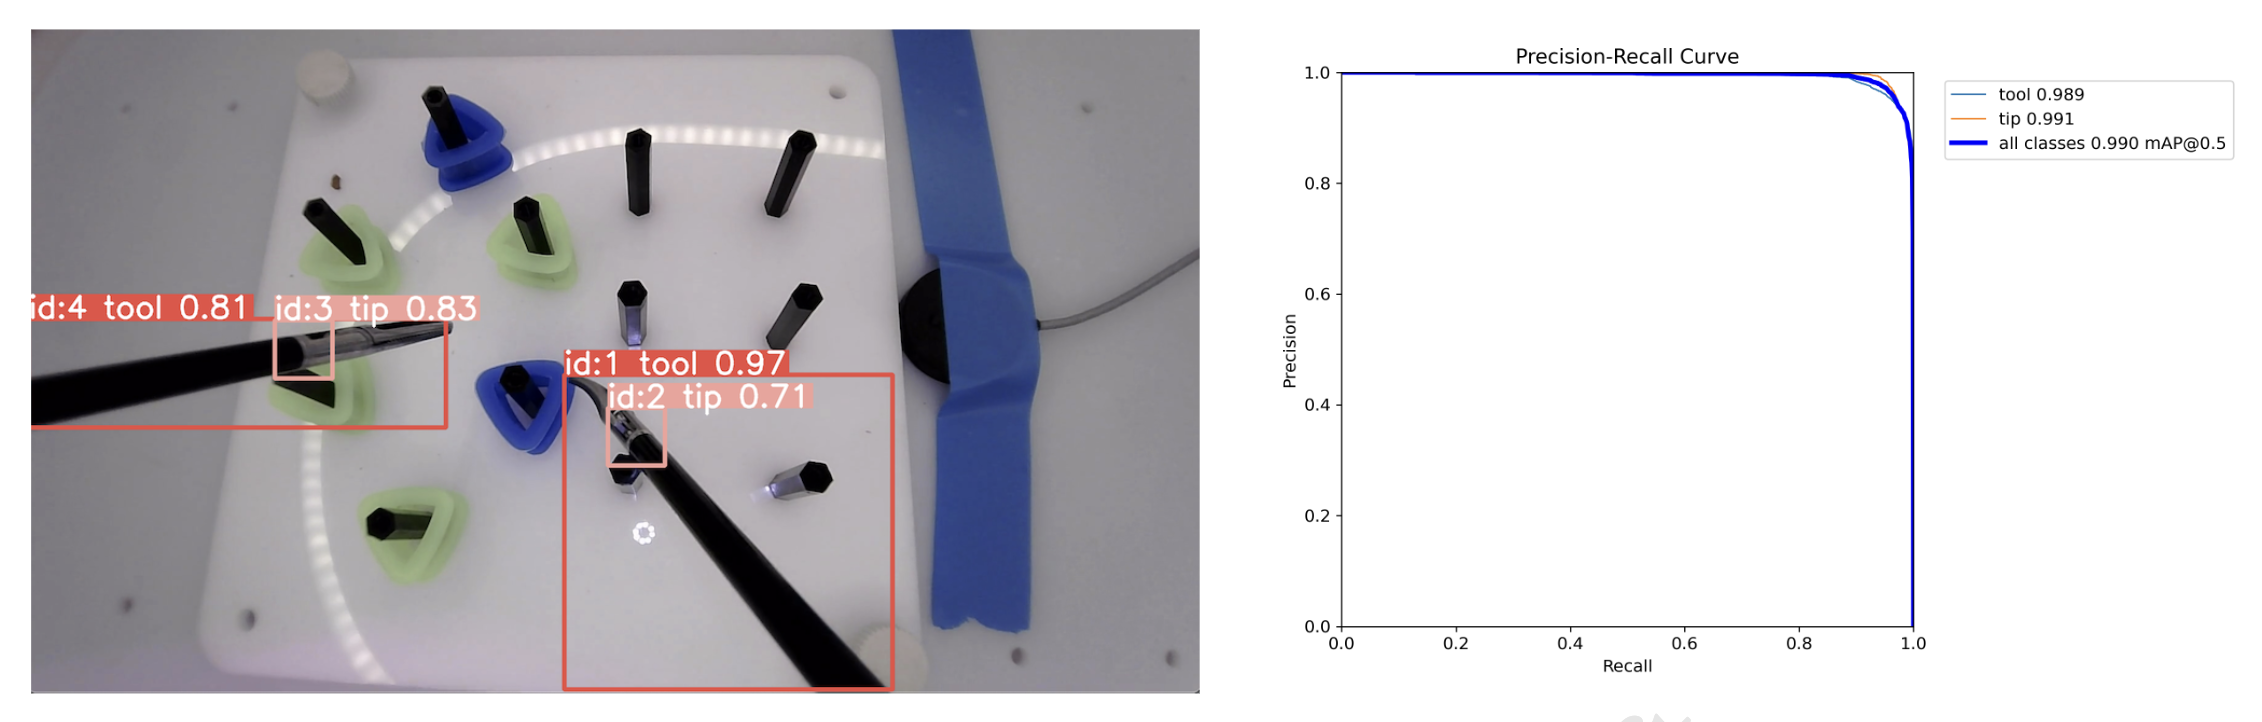
\includegraphics[height=150px]{teaserimage}
  \caption{Sample frame with tracked tools using best model and its performance.}
  \DescriptionSample{Sample frame from our dataset showing the tracked fenestrated and curved forceps and their respective tips \textit{(left)}. A plot showing the precision-recall curve for the model's performance \textit{(right)}.}
  \label{fig:teaser}
\end{teaserfigure}

\received[Submitted]{30 August 2024}
% \received[revised]{12 March 2009}
% \received[accepted]{5 June 2009}
%%
%% This command processes the author and affiliation and title
%% information and builds the first part of the formatted document.
\maketitle

% SECTION 1
\section{Introduction}

\subsection{Minimally Invasive Surgery}

Minimally Invasive Surgery (MIS) represents a significant advancement in surgical procedures by minimising tissue damage and reducing complications \cite{jaffray_minimally_2005}. Laparoscopy, a subset of MIS, involves the insertion of a laparoscope — a long, thin tube with high-intensity light and a high-resolution camera at the front — into the abdomen through a small incision, allowing surgeons to view and operate on the internal organs more precisely \cite{monnet_laparoscopy_2003}. Laparoscopy is an attractive option, particularly in resource-constrained environments (RCEs) where hospital stays and postoperative care can be expensive and logistically challenging \cite{rockall_laparoscopy_2014}. However, adopting MIS is often hindered by the scarcity of skilled surgeons, the high cost of laparoscopic equipment \cite{meara_global_2015}, and the surgeon must deal with difficult hand-eye coordination, restricted mobility and a narrow field of view, inevitably resulting in poorer quality data \cite{bodenstedt_comparative_2018}. Despite these challenges, laparoscopy remains the preferred method for many surgeries due to its benefits, such as reduced blood loss, lower infection rates, and faster recovery times than open surgery \cite{jaffray_minimally_2005}.

\subsubsection{Low and Middle-Income Countries}

In 2015, the Lancet Commission on Global Surgery emphasised the urgent need for increased volume and quality of surgery as an essential part of global health \cite{meara_global_2015}. Significant disparities in access to surgical care in LMICs contribute to an estimated 5 billion people lacking safe and affordable surgical services, with an additional 143 million surgeries annually needed to fill this gap. Furthermore, the World Health Organization has highlighted a global shortfall of 44.5 million health workers, with a considerable proportion of this deficit being in surgery \cite{world_health_organization_world_2016}. This shortage of skilled surgeons in LMICs is a substantial barrier to improving surgical outcomes and reducing the burden of surgical diseases in these regions. 

%%The Lancet Commission on Global Surgery (LCoGS) 2015 emphasised the urgent need for increased volume and quality of surgery as an essential part of global health \cite{meara_global_2015}. It recognised that developing safe, essential, life-saving surgical care in low- and middle-income countries (LMICs) has lagged behind developed nations and requires significant expansion. Significant disparities in access to surgical care compared to high-income countries (HICs) contribute to an estimated 5 billion people lacking safe and affordable surgical services, with an additional 143 million surgeries annually needed to fill this gap. 11\% of deaths in LMICs are due to conditions treatable by surgery, with 80\% of them being preventable. Furthermore, the World Health Organization (WHO) has highlighted a global shortfall of 44.5 million health workers, with a considerable proportion of this deficit being in surgery and anaesthesia \cite{world_health_organization_world_2016}. This shortage of skilled surgeons in LMICs is a substantial barrier to improving surgical outcomes and reducing the burden of surgical diseases in these regions. 

\subsection{Surgical Skill Assessment}

The global shortage of skilled surgeons significantly impacts patient outcomes, with wide variability in surgical skills leading to complications and avoidable harm \cite{jin_tool_2018}. Assessing operative skills is essential to improving surgical training. Traditional skill assessment methods are time-consuming, subjective, often rely on expert surgeons to evaluate the performance of an entire operation manually \cite{vassiliou_global_2005, paley_crowdsourced_2021} and are prone to human bias \cite{levin_automated_2019}. There is a growing emphasis on developing automated real-time surgical tool detection and tracking systems to address these limitations, offering objective and consistent evaluations \cite{loza_realtime_2024}. Various computer vision applications for tooltip detection and tracking have been developed for laparoscopic surgery training \cite{matsumoto_laparoscopic_2022}. Detection, tracking, localisation, and pose estimation techniques using computer vision and Artificial Intelligence (AI) could provide insight into surgical performance \cite{bodenstedt_comparative_2018, allan_toward_2013, constable_enhancing_2024}. Tooltip motion primitives may directly correlate to improving skill \cite{retrosi_motion_2015}. This establishes the motivation to develop models which accurately detect and track surgical tools in laparoscopic videos for use in the computer-assisted intervention of skill assessment in LMICs \cite{nwoye_cholectrack20_2023}. 
% These tools have the potential to provide feedback to trainee surgeons, investigate the aspects of skill linked to patient outcomes, and assist educators in determining if trainees meet competency thresholds.

\subsection{Objectives}

The primary objective of this study is to detect and track surgical tools using various SOTA models on the in-house Artificial Intelligence Enhanced Laparoscopic Training (AI-ELT) dataset to aid future research in in-vitro laparoscopic datasets in RCEs.

\subsection{Contributions}

We can summarise our contributions as follows:

\begin{itemize}[noitemsep, left=0pt]
\item We introduce a novel dataset of laparoscopic training videos, AI-ELT, the first of its kind for surgical skill analysis in non-in-vivo contexts with abundant high-quality annotations.
\item We develop and compare SOTA deep learning models for tool detection in laparoscopic videos, focusing on anchor-based and anchor-free architectures, inference times and model complexity.
% \item We develop and compare SOTA deep learning models for surgical tool detection in laparoscopic videos, focusing on anchor-based and anchor-free architectures, inference times and model complexity, providing valuable insights for future research in surgical training in RCEs.
\item We develop a surgical tool tracking algorithm for the AI-ELT dataset, achieving 100\% accuracy over already detected tools and tooltips, setting a foundation for real-time feedback and skill assessment in surgical training programs.
\end{itemize}

% TABLE OF ACRONYMS
% \begin{table}[h]
%     \centering
%     \caption{Table of Acronyms}
%     \begin{tabular}{ll}
%       \toprule
%       \textbf{Acronym} & \textbf{Definition} \\
%       \midrule
%       6DoF & Six Degrees-of-Freedom \\
%       AI & Artificial Intelligence \\
%       AI-ELT & AI Enhanced Laparoscopic Training \\
%       COCO & Common Objects in Context \\
%       FPS & Frames Per Second \\
%       HICs & High-Income Countries \\
%       IoU & Intersection over Union \\
%       LCoGS & Lancet Commission on Global Surgery \\
%       LMICs & Low and Middle-Income Countries \\
%       MIS & Minimally Invasive Surgery \\
%       mAP & Mean Average Precision \\
%       SOTA & State-of-the-Art \\
%       WHO & World Health Organization \\
%       \bottomrule
%     \end{tabular}
%     \label{tab:acronyms}
%   \end{table}


% SECTION 2
\section{Related Work}

\subsection{Literature Search}

The search strategy was meticulously designed to ensure a comprehensive and thorough exploration of the literature concerning surgical tool tracking and related topics. The selected databases — PubMed and Ovid - are among the most comprehensive resources for biomedical literature, ensuring that the search covers a broad spectrum of relevant research. The literature search began in April, and to keep the review current, alerts were set up on PubMed to capture any newly published research. This ongoing search process, combined with backward and forward citation tracking and additional searches through other sources like Google Scholar, ensured that the review was as comprehensive and up-to-date as possible.

The Figure \ref{fig:prisma} illustrates the flow of the search and inclusion process, following the recommendations of the Preferred Reporting Items for Systematic Reviews and Meta-Analyses (PRISMA) statement \cite{moher_preferred_2010}. The strategy was divided into three main categories: tool-related searches, skill-related searches, and segmentation-related searches. This was not focused on conducting a systematic review but rather on establishing context, considering state-of-the-art (SOTA) methods and models, and identifying areas for further research in AI-enhanced laparoscopic training. This approach allows for a more flexible and comprehensive understanding of the current research landscape, facilitating the identification of gaps and opportunities for future research, including the focus for this study.

\begin{figure}[htbp]
    \centering
    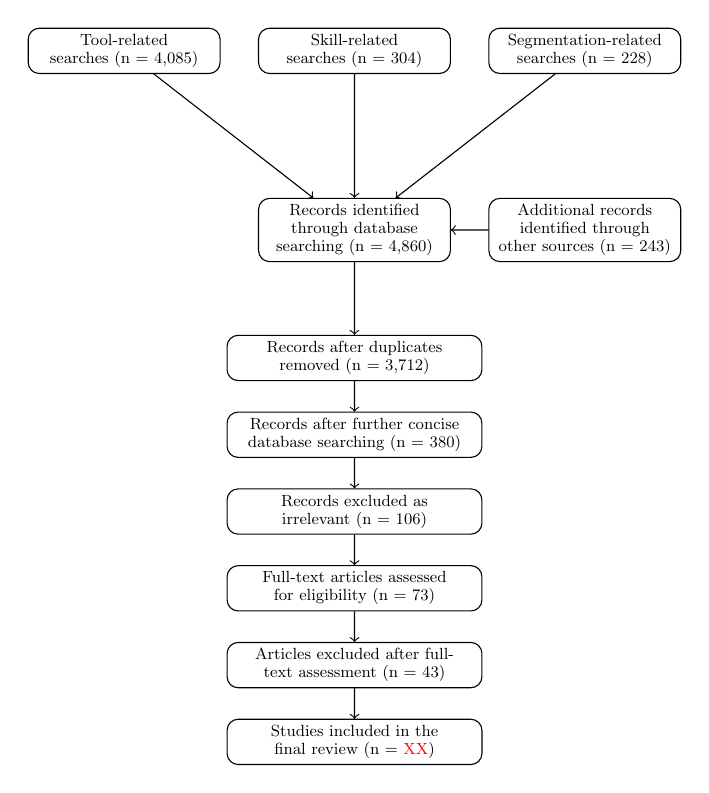
\begin{tikzpicture}[node distance=1.5cm, scale=0.65, every node/.style={transform shape, font=\fontsize{9}{10}\selectfont}]

    % Top level boxes
    \node (tool) [rectangle, draw, text width=10em, text centered, rounded corners] {Tool-related searches (n = 4,085)};
    \node (skill) [rectangle, draw, text width=10em, text centered, rounded corners, right of=tool, xshift=3cm] {Skill-related searches (n = 304)};
    \node (segmentation) [rectangle, draw, text width=10em, text centered, rounded corners, right of=skill, xshift=3cm] {Segmentation-related searches (n = 228)};

    % Box connecting to database searching
    \node (id) [rectangle, draw, text width=10em, text centered, rounded corners, below of=skill, yshift=-2cm] {Records identified through database searching (n = 4,860)};
    \draw[->] (tool) -- (id);
    \draw[->] (skill) -- (id);
    \draw[->] (segmentation) -- (id);

    % Additional records
    \node (os) [rectangle, draw, text width=10em, text centered, rounded corners, right of=id, xshift=3cm] {Additional records identified through other sources (n = 243)};
    \draw[->] (os) -- (id);

    % Duplicates removed
    \node (dup) [rectangle, draw, text width=13.5em, text centered, rounded corners, below of=id, yshift=-1cm] {Records after duplicates removed (n = 3,712)};
    \draw[->] (id) -- (dup);

    % Screening
    \node (sc) [rectangle, draw, text width=13.5em, text centered, rounded corners, below of=dup] {Records after further concise database searching (n = 380)};
    \draw[->] (dup) -- (sc);

    % Irrelevant exclusion
    \node (ex) [rectangle, draw, text width=13.5em, text centered, rounded corners, below of=sc] {Records excluded as irrelevant (n = 106)};
    \draw[->] (sc) -- (ex);

    % Full text assessed
    \node (ft) [rectangle, draw, text width=13.5em, text centered, rounded corners, below of=ex] {Full-text articles assessed for eligibility (n = 73)};
    \draw[->] (ex) -- (ft);

    % Articles excluded after full text assessment
    \node (fa) [rectangle, draw, text width=13.5em, text centered, rounded corners, below of=ft] {Articles excluded after full-text assessment (n = 43)};
    \draw[->] (ft) -- (fa);

    % Final studies included
    \node (inc) [rectangle, draw, text width=13.5em, text centered, rounded corners, below of=fa] {Studies included in the final review (n = \textcolor{red}{XX})};
    \draw[->] (fa) -- (inc);

    \end{tikzpicture}
    \caption{PRISMA Flow Diagram}
    \Description{The flow diagram of the paper selection and pruning process according to the recommendations of the PRISMA method.}
    \label{fig:prisma}
\end{figure}

\subsection{Identification and Evaluation of Relevant Datasets}

We identified 64 surgical datasets, of which we categorised 5 for tracking (where there is video access or subsequent frames available with appropriate annotations), 4 for pose estimation (with ground truth sensor data), 6 for detection (only bounding box annotations available), 10 for skill (classification of the operators' surgical skills), 11 for workflow analysis (the current sub-procedure or workflow carried out by the surgeon), 20 for segmentation (with full tool masks) and 7 for other use. Since some datasets have multiple use cases, we organised them so that if we could use them for tracking then we considered it to a dataset for tracking. In total, 37 datasets were identified as being useful with 9 excluded as they were based on robotic surgery (not relevant to us), with the remaning 18 datasets being excluded as they were not relevant. Only 7 datasets were ready for immediate use, with a further 5 available after requesting access.

Some datasets had more value as the quality of images and annotations were greater and very few had code available for direct use. We list these datasets as follows: MICCAI 2015 Endoscopic Vision Challenge (EndoVis 2015), MICCAI 2016 Endoscopic Vision Challenge (m2cai16), MICCAI 2024 Endoscopic Vision Challenge (SurgVU) \footnote{Based on the previous 2022 and 2023 challenge versions.}, PEg TRAnsfer Workflow Recognition by different modalities (PETRAW) \footnote{Sub-challenge as a part of MICCAI 2021} and the Augmented Reality Tool Network (ART-Net) dataset. Of these, the most relevant datasets were PETRAW as it is the ideal quality of the dataset that we would expect ours to be and ART-Net as it contained segmentation masks for tooltips which is something most datasets lacked.

% avoiding segmentation

% ART-NET: If there is enough time, we could try the method on another dataset. For ART-Net, we could convert the segmentation map into a bounding box, for the entire tool and just for the tool tip. I could consider other public datasets and what has been benchmarked already and how, so that I could employ the same method for comparison.

\subsubsection{Potential to Collect New Datasets}

% training datasets are fewer, easier to collect and to be used in LMIC

\subsection{State-of-the-Art Object Detection Methods}

% emphases what has been done

% Anchor-based is interesting because videos often have a wide range of aspect ratios, etc. (insert examples). We decided that it would be best to continue with the current dataset, and to make it scientific and sufficient for the MSc, I would look at investigating anchor-based methods (e.g. YOLO) and anchor-less methods (fully connected one-stage CNN). A method for each would be sufficient. The idea is that the aspect ratio of the tool will change as it moves around and is rotated, with different orientations and scales in various ways, so anchors in anchor-based methods would need to be optimised. I would look at what methods could cope with those situations and what their limitations are.

% Many Deep Learning based methods such as Fast-RCNN have achieved SOTA performance in tool detection and localization (Du et al, 2018a) but are computationally expensive, introducing inference time penalties. https://arxiv.org/abs/2209.01435

We can use RetinaNet with anchor-box optimisation \cite{zlocha2019improving}.

\subsection{Tracking Methods}

% Secondary focus is tracking, the main focus is on detection. Tracking can be done if IDs are tracked and we consider tools moving out of frame (their appearance, disappearance and reappearance). Segmentation is not needed as tracking is our aim, not pixel-wise classification.

% many different algorithms, and list some (DeepSORT, ByteTrack, BotSORT) however we will create our own algorithm for us on datasets similar to PETRAW and our dataset.

\subsubsection{Computer Vision Methods}

There are many alternative methods which can be used for specific tasks, which can be incredibly useful with increasing accuracies of detection and tracking. Optical flow methods estimate the motion of objects between consecutive frames of video. By tracking keypoints or pixels, these methods can determine movement patterns which correspond to the movement of the tool. A key technique used in the Lucas-Kanade method which utilises a differental method for optical flow estimation, efficient for small motion which is what we experience in laparoscopic data. It also uses the Horn-Schunkck method which assumes smoothness in the motion field. This works well in real-time applications and can be used to track movement across frames with moderate accuracy. We can improve the robustness and accuracy by using sensor data to initialise and help guide the optical flow tracking process. The Kalman Filter method is an extremely popular and widely used method in tracking which provides estimates of unkown variables by optimally combining a series of measurements observed over time, which is excellent for real-time applications and noisy data. A particle filter can track the tool positions based on probabilistic models, based on sensor readings and a motion model. This makes it robust to non-linearities and multi-modal distirbutions in the sensor data. Background subtraction is a simple method which involves separating foreground objects from the background in video frames to isolate and track moving objects. We can use Gaussian Mixture Models to model the background using multiple normal distributions to adapt to changes in lighting, scene dynamics and camera movement. The simplest methd is to use frame differencing to highlight moving objects. This is extremely effective in controlled environments with static backgrounds making it highly suitable in our application. Feature matching can be used to track movement by detecting and matching key features such as corners and edges. With enhancemnets such as speeded-up robust features (SURF), a faster alternative to scale-invariant feature transform (SIFT) which describes local features, we can track keypoints in real-time applications, robust to scale and rotation changes common in laparoscopic videos. We could use template matching where we use pre-defined templates of the tools to locate and track frame-by-frame. Its weakness is in aspect-ratio changes which can be countered by also implemeneting one of the aforementioned SIFT or SURF techniques. Simple edge detection and contour tracking can also be used in non in-vivo datasets where there is a simpler non-moving background compared to in-vivo data.

\subsubsection{Artificial Intelligence Methods}

Artificial intelligence methods can be used to track tools in laparoscopic videos. We can use a deep learning method such as a convolutional neural network (CNN) to detect tools in images. Then we can use a recurrent neural network (RNN) to use previous information to help reinforce predictions in the current frame. We coudl also use a long short-term memory (LSTM) network to remember information over long periods of time, or a gated recurrent unit (GRU) network which is a simplified version of an LSTM network which is more efficient and can be used in real-time applications. We could use a transformer network which is a deep learning model that uses attention mechanisms to learn dependencies between input and output data. 
All of these methods essentially allow us to track tools in real-time applications, with the ability to learn from previous frames and predict future frames.

\subsection{Potential Gaps and Insights}

% what has not been done whicih could be done
% pose research questions

\subsection{Limitations}

\subsection{Future Use Cases}

% Need to have a concise plan going forward. I have focused on image tracking and segmentation across many datasets. Going forward, I should consider what could be done, working with state-of-the-art (SOTAs) and focusing on something different to give different results. Using the papers from the literature review I have carried out, I should pick a paper, run the SOTA method and consider why it performs best or why it fails at certain things. These things are where I should look for improvements. Consider the mistakes made and how I could solve them. If there are good and bad samples, then focus on those which fail and innovate on what could be done about them. For example, there could be different sizes or occlusions or look at the domain-safe problem (solving the generalisation problem on real and fake data). If the methods do not work on real data, what is the gap which needs to be solved? Goal is to get inference down.

% SECTION 3
\section{Methodology}

\subsection{Datasets}

\subsubsection{AI-ELT}

Our in-house dataset was collected on 11-12th October 2023 at the 8th Urology Boot Camp in Leeds, United Kingdom \cite{urology2023}. It contains 24 videos, each a procedure performed by a single participant. All participants, surgical trainees and trainers were given a handout, as shown in Figure \ref{fig:dataset-collection}, which explained the study and the data collection process. We used a Simulated Insufflated Belly Laparoscopic Trainer Simulator Training Box with 30 Degree 1920x1080 HD Camera. The sensors were three NDI Aurora 6DoF (Six Degrees-of-Freedom) electromagnetic trackers (one on each tool and one on the camera). The calibrated position was to the fulcrum of each tool, performed by pivot calibration (see the black sensor on the right of the peg transfer board with the blue tape in Figure \ref{fig:test1_issues}). Handedness data was collected using the Edinburgh Handedness survey in various other tasks, including writing, drawing, throwing, scissors, toothbrush, knife (without fork), spoon, broom (upper hand), striking a match (hand holding match) and opening a lid (hand opening lid) \cite{oldfield_assessment_1971}. Level of expertise was estimated using the number of procedures in their lifetimes and within the last 12 months. Participants were confirmed not to have a pacemaker or other metal implants which could interfere with the electromagnetic tracking system. In this study, there was no need for any participant follow-up.

% Generally compared to other datasets, the camera was of higher resolution with increased field-of-vision (FOV), contained two tools in all procedures (many laparoscopic videos contain just a single tool), and 6DoF ground truth three-dimensional tooltip positions and spatial rotation quaternions. Surgeon information included data about the participants' handedness and level of expertise.

\begin{figure}[htbp]
    \centering
    \vspace*{-6mm}
    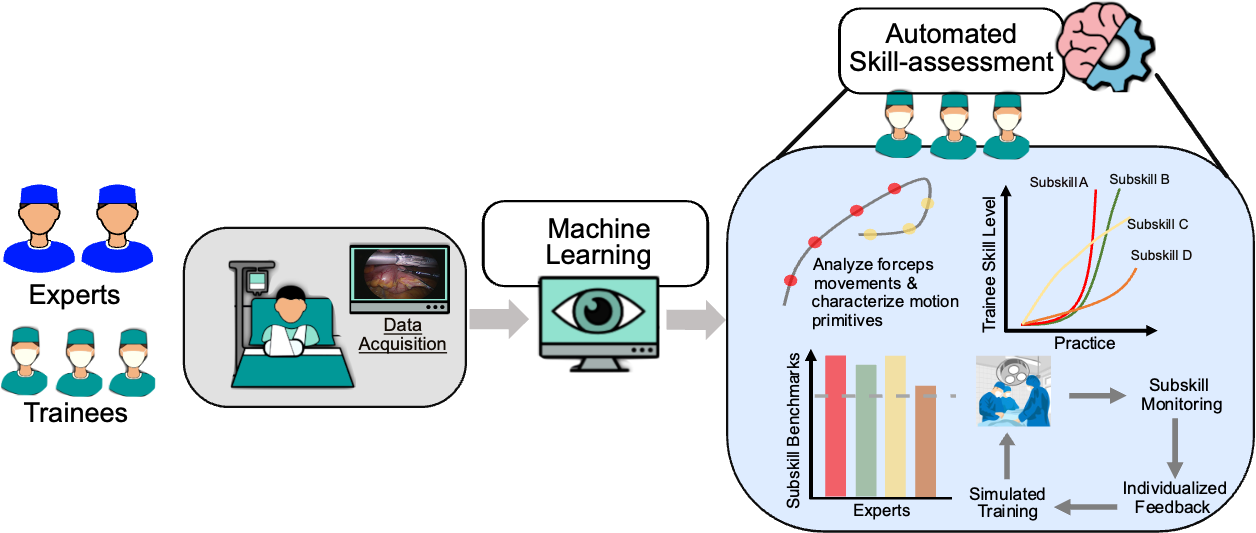
\includegraphics[width=1\linewidth]{dataset_collection.png}
    \vspace*{-6.5mm}
    \caption{AI-ELT Dataset Collection}
    \vspace*{-3mm}
    \label{fig:dataset-collection}
    \Description{Handout given to surgeons preceding the data collection process.}
\end{figure}

% The handout explained that the study was to collect motion data from a peg transfer task. The goal was to train an AI system to localise the laparoscopic tools using the image alone. This would help develop a new training system, giving automated feedback on individual sub-skills. In this study, we focused on first detecting the tools, which could then be used with the sensor data to build a model which could predict the tools' motion based on the tool's location in the image.

The final dataset comprises 24 laparoscopic surgery videos, each approximately 3 minutes long in 1920x1080 resolution, totalling 1.32GB. These videos feature procedures performed by either a trainee or an expert trainer. The dataset includes 103,629 frames annotated with the 6DoF ground truth data. The first trial contained extra lighting causing visual defects (see Figure \ref{fig:test1_issues}), which was removed for subsequent trials.

\begin{figure}[htbp]
    \centering
    \vspace{-3mm}
    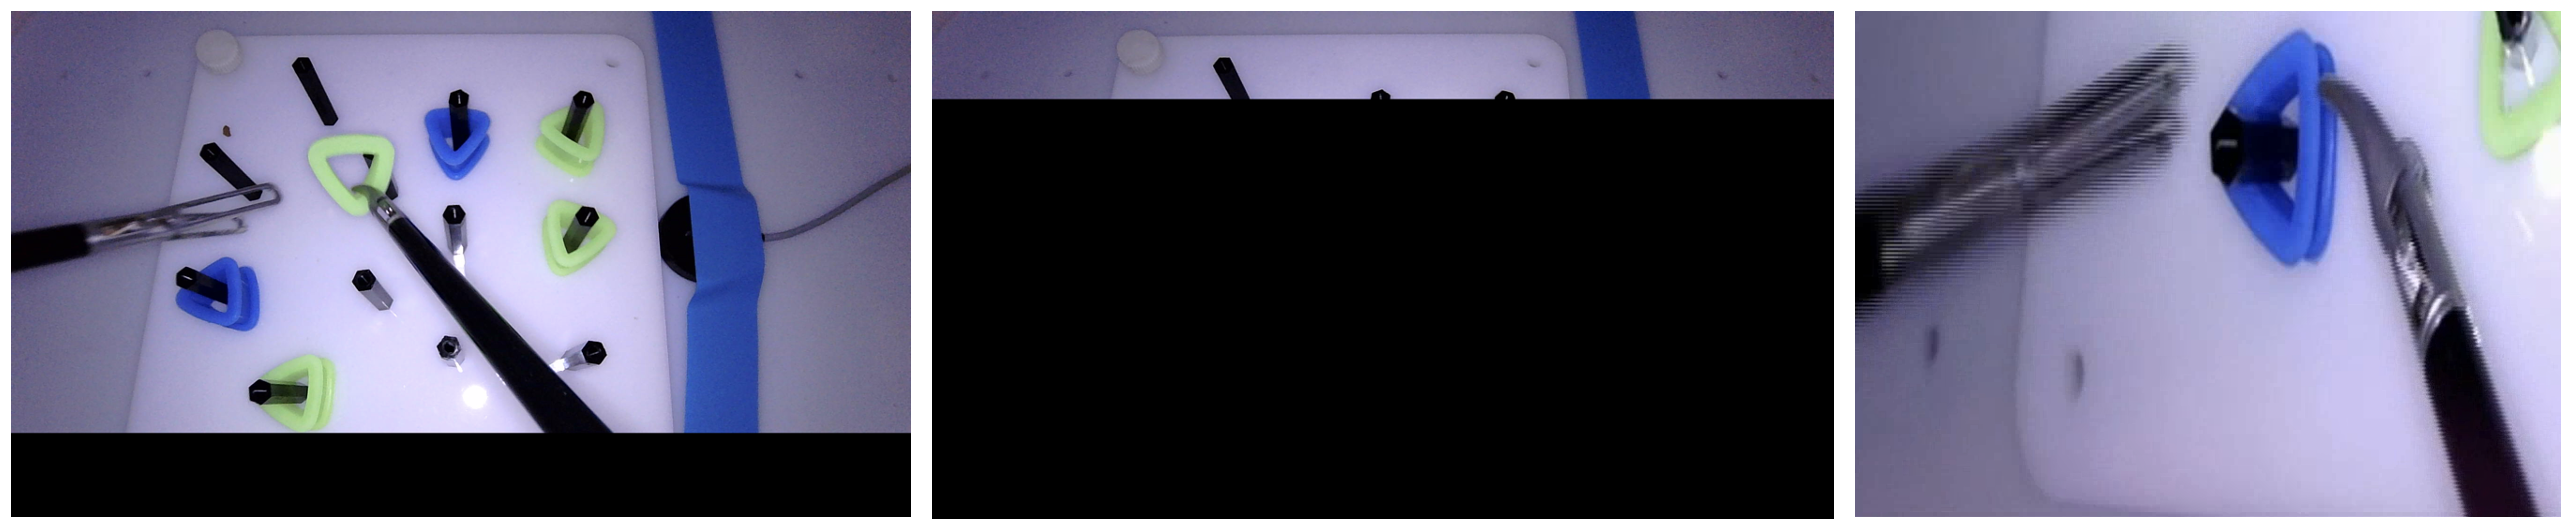
\includegraphics[width=1\linewidth]{test1_issues}
    \vspace*{-7.5mm}
    \caption{Issues with the dataset}
    \vspace*{-5mm}
    \label{fig:test1_issues}
    \Description{We see a few issues with the dataset. Of all 24 videos, 1 emits extra light onto the scene (Test 1). We also see some frames have been cut off, either a little (\textit{left}) or a lot (\textit{middle}). We also note some camera overheating, causing image defects (\textit{right}).}
\end{figure}

% The average number of procedures performed was 120, with a range of 0 to over 1000, with 22 estimated to be performed on average in the last 12 months, ranging from 0 to 100. All 24 participants agreed to share their results entirely. If we categorise the surgeon's skills based on several procedures, where low is <20, medium is between 20 and 100, and high is >100, then we have 9 low, 9 medium and 6 high-skilled surgeons. Results from the Edinburgh Handedness survey \cite{oldfield_assessment_1971} showed almost all surgeons were right-handed, with one left (participant 12) and one who alternated hands (participant 3).

% The results of the Edinburgh Handedness survey \cite{oldfield_assessment_1971} could be used to evaluate surgical skills based on the handedness of the surgeon. Further annotations could be developed based on existing metrics of technical surgeons, e.g. Objective Structured Assessment of Technical Skills (OSATS) \cite{martin_objective_1997, hussein_development_2017}. Though based on questionnaires and subjective, they could help set a baseline for categorising surgical skill level \cite{hilal_randomized_2017}. Key movement metrics which define the skill level for typical tasks in a laparoscopic procedure can be identified \cite{pears_capturing_2021}. These metrics can be quantified from trainee videos to create task-specific learning curves.

\subsubsection{Data Preparation}

Inspired by the CholecTrack20 schematic diagram, we present an intuitive way to understand the dataset \cite{nwoye_cholectrack20_2023}.

\begin{figure}[htbp]
    \centering
    \vspace*{-2mm}
    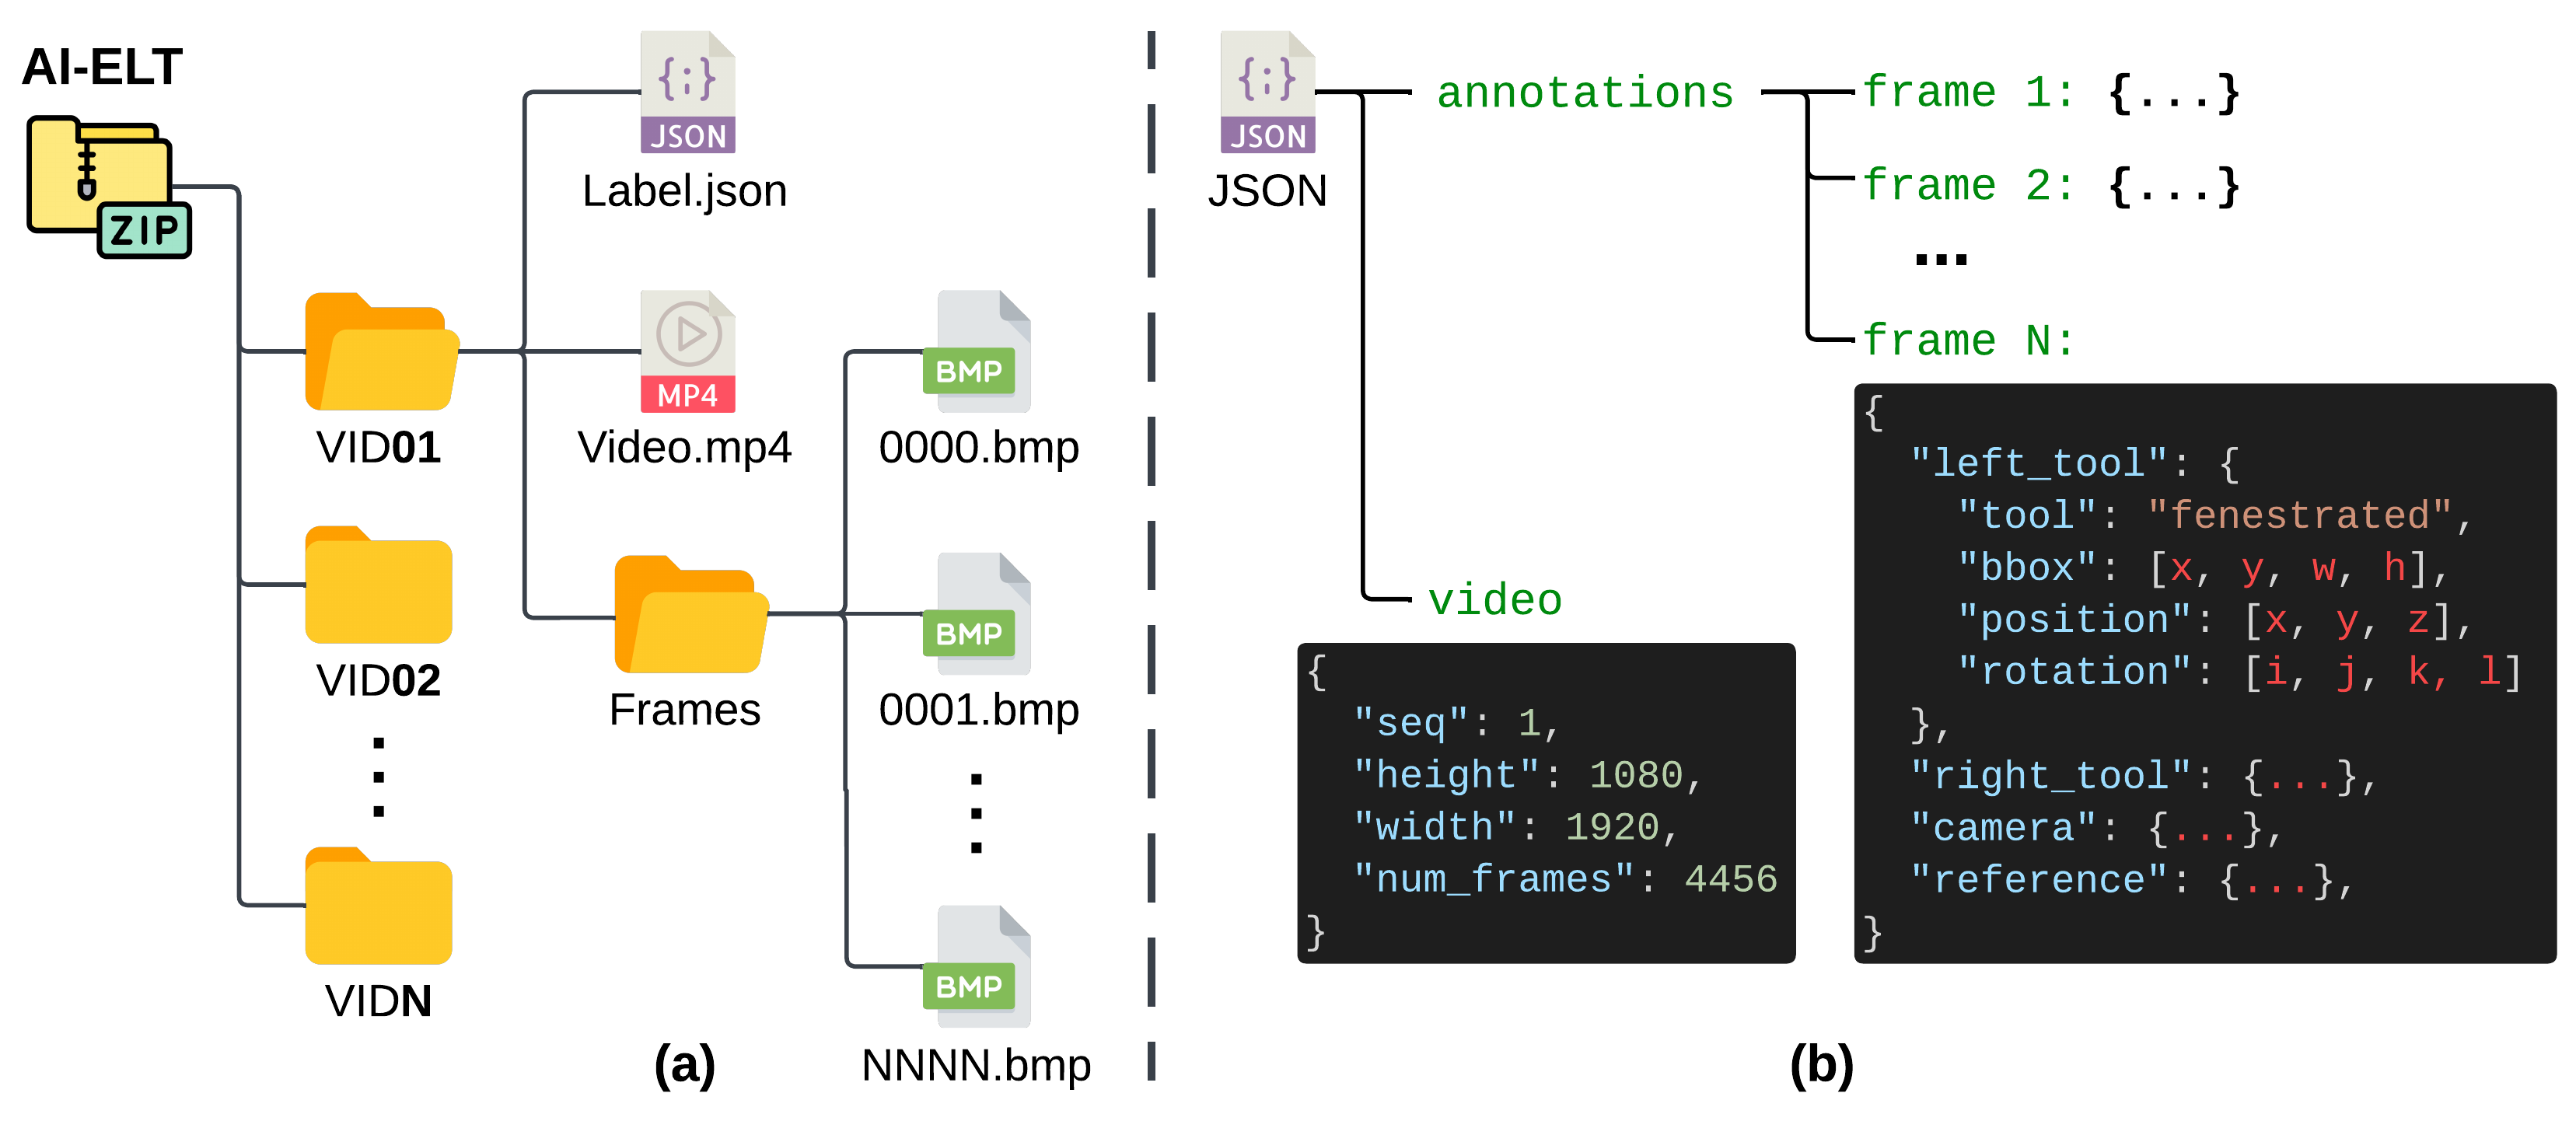
\includegraphics[width=\linewidth]{schematic_diagram.png}
    \vspace*{-7.5mm}
    \caption{Schematic diagram of the dataset files showing (a) folder structure for the dataset and (b) Data structure for the JSON label files.}
    \vspace*{-2.5mm}
    \label{fig:schematic_diagram}
    \Description{Schematic diagram for the AI-ELT Dataset}
\end{figure}

To ensure robust model validation, we have manually labelled 1\% of the images across 23 videos and one video fully labelled as a test set (Video 5) by modifying an existing keypoint annotation tool \cite{herrera_luiscarlosgphkeypoint-annotation-tool_2024}. Annotations were recorded in Common Object in Context (COCO) format with class (either tool or tooltip), bounding box centre ($x$), bounding box centre ($y$), width and height. No duplicates, outliers or inconsistencies were noticed. However, we see a few issues with the dataset (Figure \ref{fig:test1_issues}). Some frames have been cut off, either a little (\textit{left}) or a lot (\textit{middle}). We also note some camera overheating, causing image defects (\textit{right}). We appropriately removed missing data for model training, giving 864 clean training data files out of 1045.

Our code contains multiple helper functions and classes to assist in future development \cite{choudhry_omarioscmsc-surgical-tool-tracking_2024}. This will be adapted to a more formal AI-ELT framework in the future. Before manual annotation, we attempted to get the objects' $x$ and $y$ positions using ground truth 3D position data, matrix transformations with intrinsic and extrinsic camera and scene parameters, and regular linear regression. However, the error margin was too high. The best-produced model could be used to annotate remaining bounding boxes with weak labels in a teacher-student framework or for a more complex model to reverse-engineer positions from motion data in future datasets \cite{teevno_semi-supervised_2023}.

\subsubsection{Other Datasets}

The final decision was to perform additional extensive evaluation solely on the ART-Net dataset \cite{hasan_detection_2021}. Since we will re-implement the ART-Net model (with its code already available), it is logical to use the same dataset to evaluate the reproducibility and a more objective evaluation of the methods by comparing results. We converted the ART-Net tool and tooltip segmentation maps to bounding boxes (1,324 training images and 308 test images). We will keep the datasets' negative examples, which do not contain any tools to attempt to reduce potential false positives.

\subsection{Reimplementation of the State-of-the-Art}

Multiple anchor-based and anchor-free deep learning SOTA models are implemented and tested to consider LMIC resource constraints. The models were trained on a system with the following configuration: AMD Ryzen 3900X CPU, 32GB RAM, and an NVIDIA GeForce RTX 3060 GPU with 12GB of memory, running on Windows 11 Pro with PyTorch 2.2.1+cu121. In practice, the goal is to ensure these models can eventually be deployed on even less powerful and more affordable hardware. We use transfer learning by fine-tuning models with SOTA checkpoints to reduce training times and multiclass and multitask learning to meet our detection requirements \cite{alabi_multitask_2024}.

\subsubsection{Anchor-based Object Detection}

We tested all six different architectures of YOLOv10 (X, L, B, M, S, N). We tested various architectures to investigate the effect of parameters and architecture size on inference and precision. RetinaNet and EfficientDet were trained with their default configurations. We also ran RetinaNet with anchor-box scale and ratio optimisation \cite{zlocha_improving_2019}.

\subsubsection{Anchor-free Object Detection}

The anchor-free models we tested were all five different architectures of YOLOv8 (X, L, M, S, N), the Single Input Multiple Output (SIMO) ART-Net model (with a ResNet 50 backbone for faster inference \cite{koonce_resnet_2021} and the original VGG 16 backbone \cite{hasan_detection_2021}) and the End-to-End DEtection TRansformer (DETR). The SIMO model was implemented using Tensorflow in PyTorch with a modified final layer to output bounding box annotations for left and right tools and tips. YOLOv8 and DETR were trained with their default configurations.

\subsubsection{Tracking Algorithm}

The tracking algorithm we developed first identifies each surgical tool by checking the bottom half of its bounding box to determine the shaft axis direction — left tools exhibit a positive gradient, and right tools exhibit a negative gradient. Once a tool is identified, the tooltip detected within its bounding box inherits the tool's ID. A probabilistic model then uses previous predictions and the Euclidean distance between bounding box centres to inform decisions, ensuring consistent tracking and reidentification if a tool temporarily leaves the frame or is obscured.

\subsubsection{Model Training}

The models were trained using default configurations, ensuring consistency across different architectures and datasets. Specific hyperparameters included a batch size of 16 (8 for memory-intensive models like SIMO and EfficientDet) and patience set to 10, allowing early stopping if validation performance did not improve after 10 epochs. Inference times were calculated based on the detection times per image over the test set. The YOLOv10 models trained on the AI-ELT dataset were fine-tuned versions of the models initially trained on the ART-Net dataset, which slightly reduced the epoch numbers needed for convergence. RetinaNet models with anchor-based optimisation were also fine-tuned versions of their non-optimised counterparts. Validation testing frequency was reduced to every 10 epochs to expedite training, especially for models with longer convergence times.

% YOLO models employed a specific type of mosaic augmentation to improve generalisation, where images are cropped and stitched together to form a larger image, increasing the model's robustness to different spatial contexts. 

\subsubsection{Loss Functions and Evaluation Metrics}

These models are evaluated using the standard Common Objects in Context (COCO) metric, yielding mean Average Precision (mAP) scores for detected tool and tooltip bounding boxes. These metrics were also used in loss functions across all models. Some models had additional loss function terms, but we will not expand upon them due to conciseness. Intersection over Union (IoU) is a metric that calculates the overlap between the predicted bounding box and the ground truth bounding box. It is defined as the ratio of the intersection area to the union area of the two boxes. An IoU score of 1 indicates perfect alignment, while a score of 0 indicates no overlap. We can use $1 - IoU$ for an IoU loss. Mean Average Precision (mAP) measures the average precision across all classes at different IoU thresholds. Specifically, mAP${_50}$ refers to the mean average precision at an IoU threshold of 0.5, meaning that a predicted bounding box is considered correct if its IoU with the ground truth is greater than 0.5. mAP${_{50:95}}$ is a more stringent metric that averages the precision ($AP$) across multiple IoU thresholds (from 0.5 to 0.95 in increments of 0.05). This also allows us to produce precision and recall values.

\begin{equation}
    \text{IoU} = \frac{\text{\small{Area of Intersection}}}{\text{\small{Area of Union}}}.
\end{equation}
\begin{equation}
    \text{mAP}_{50} = \frac{1}{n} \sum_{i=1}^{n} \text{AP}_{i}(\text{IoU} > 0.5)
\end{equation}
\begin{equation}
    \text{mAP}_{50:95} = \frac{1}{41n} \sum_{t=0.5}^{0.95} \sum_{i=1}^{n} \text{AP}_{i}(\text{IoU} > t)
\end{equation}


% SECTION 4
\section{Experimentation}


% \textbf{Results:} The anchor-free YOLOv8-X model was the most accurate, achieving a mAP_{50} of 99.5\% and a mAP_{50:95} of 85.6\% on the test set with an inference time of 21.7ms, approximately 46 frames per second (FPS), demonstrating its effectiveness in real-time surgical tool detection. The most efficient model was YOLOv8-N, achieving a mAP_{50} of 99.5\% and a mAP_{50:95} of 83.3\% with 1.8ms inference time, approximately 555FPS (with only 3 million parameters - less than 20x the number in YOLOv8-X). The proposed tracking algorithm has an accuracy of 100\% over the detected tools and tooltips.
\subsection{In-House Dataset}

% describe the flow of participants throughout the study

% number of participants

% outcome overall: Clear differences in some images (see differences in Test1 and Test2 scenes, and cut off images in Test2. Overheating in camera causing some image defects. edges more distinct, exact SOTA for opposite (YOLO in IRL, SIMO for ART)	 

% summary of follow-up

% overall characteristics of data source and setting

% we further used the best performin model to generate annotations for the rest of the dataset

\begin{figure}[htbp]
    \centering
    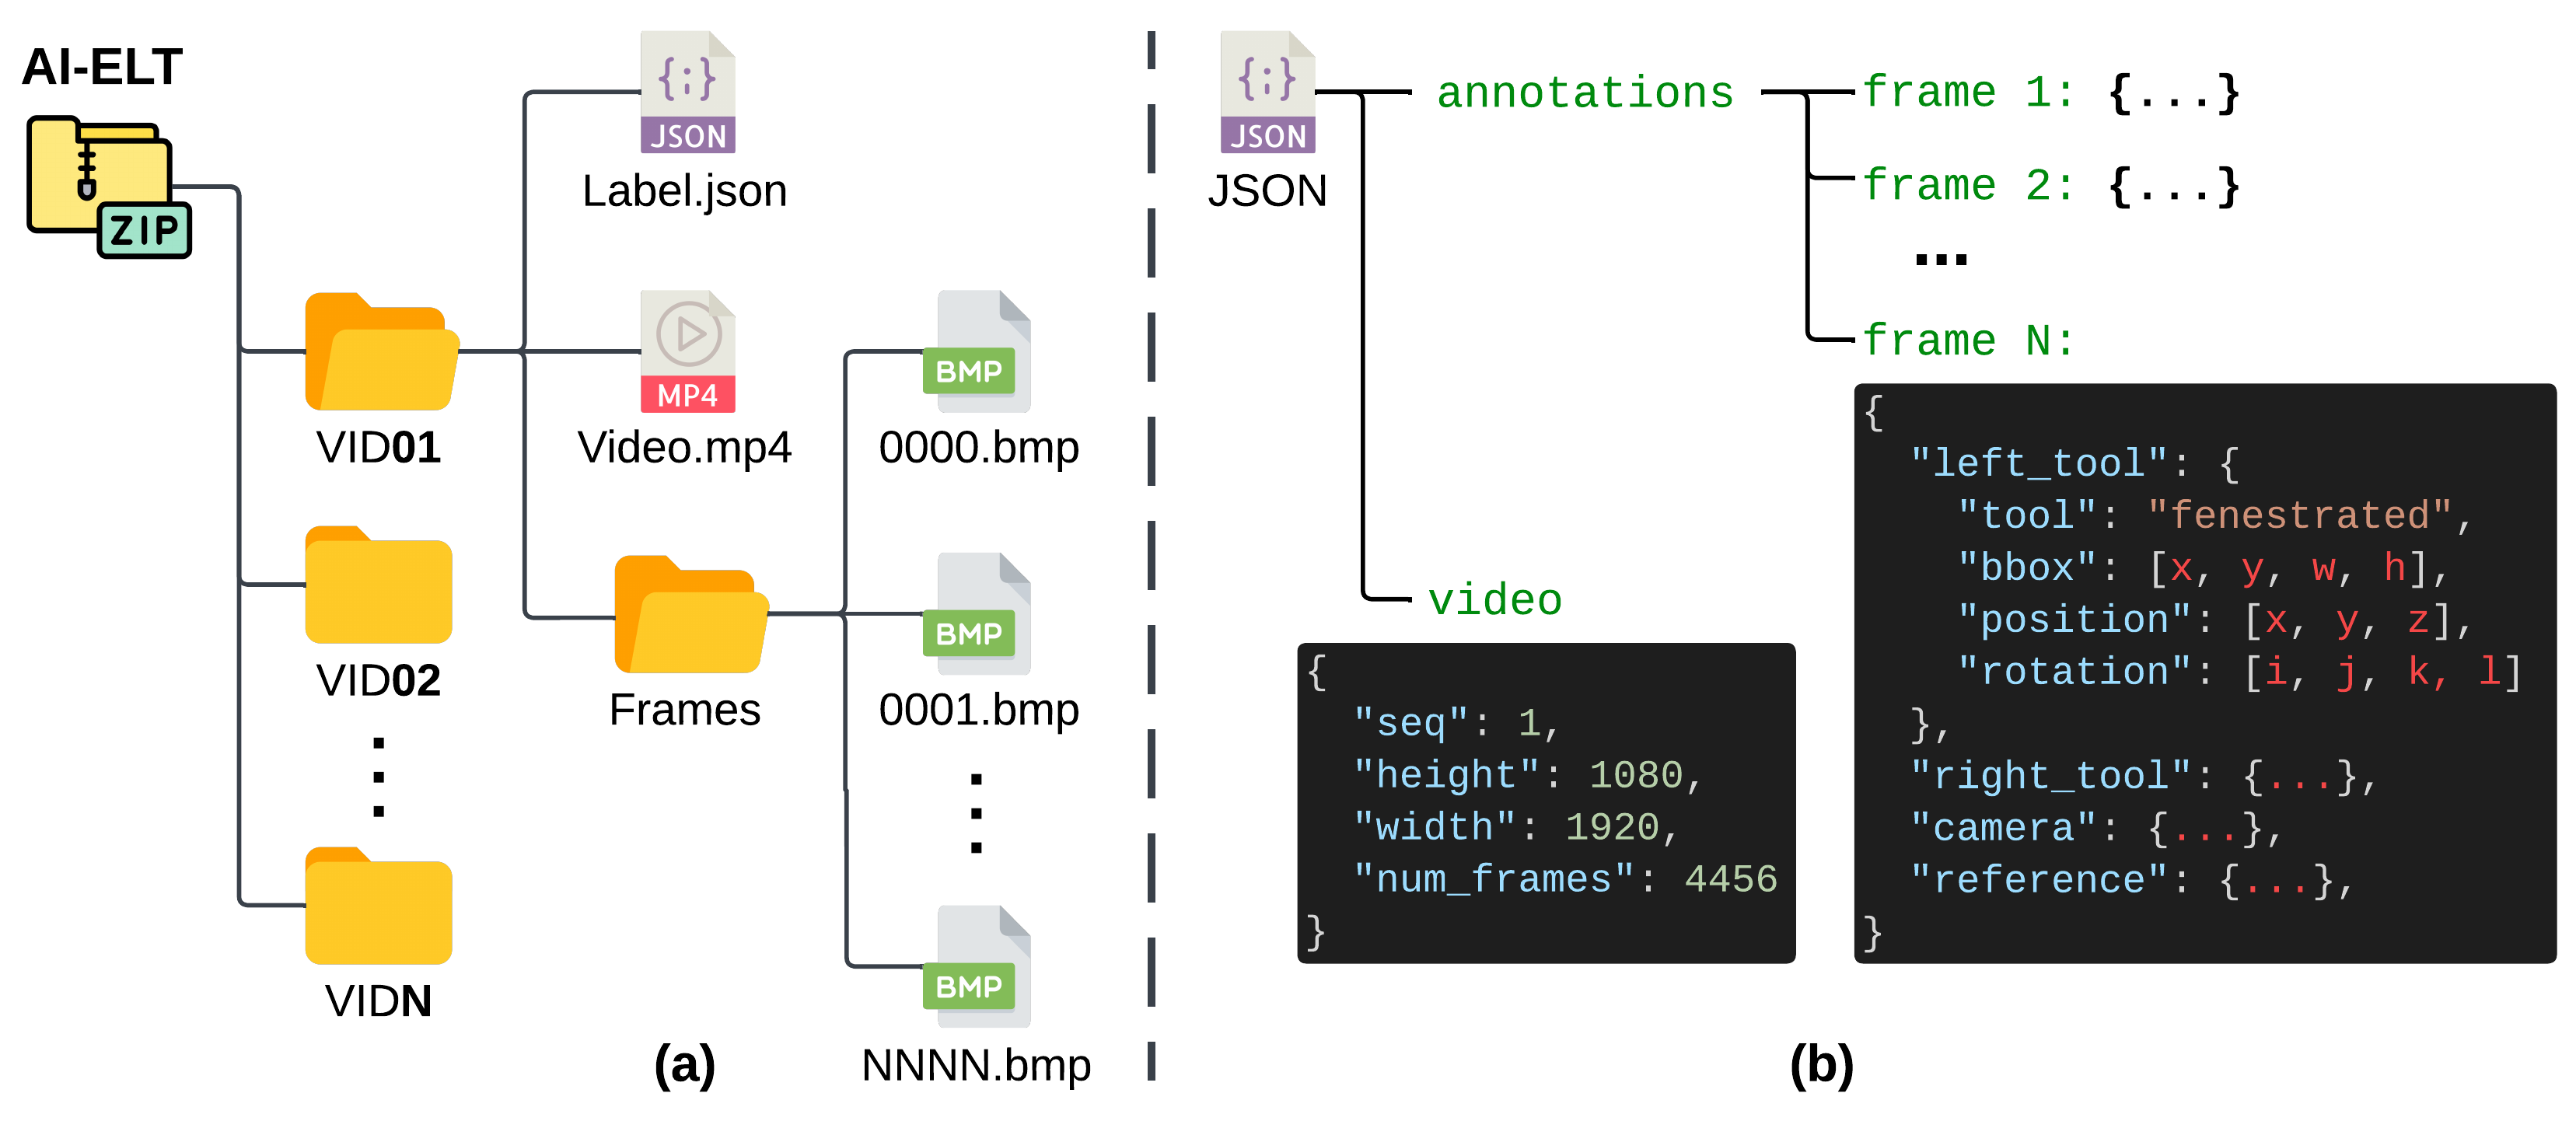
\includegraphics[width=\linewidth]{schematic_diagram.png}
    \caption{Schematic diagram of the dataset files showing (a) folder structure for the dataset and (b) Data structure for the JSON label files.}
    \label{fig:schematic_diagram}
\end{figure}

Inspired by the CholecTrack20 schematic diagram \cite{nwoye_cholectrack20_2023}, we present an intuitive way to understand the dataset.

The average number of procedures performed was 120, with a range of 0 to over a 1000, with 22 estimated to be performed on average in the last 12 months, ranging from 0 to 100. All 24 participants agreed to share their results entirely. If we categorise the surgeons skill based on number of procedures, were low is <20, medium is between 20 and 100 and high is >100, then we have 9 low, 9 medium and 6 high skilled surgeons. Results from the Edinburgh Handedness survey \cite{oldfield_assessment_1971} showed almost all surgeons were right-handed, with one left-\usepackage{multirow}
 (participant 12) and one who alternated hands (participant 3).

\subsubsection{Data Annotations}

% overall data annotated

% issues faced

In future, further annotations could be developed based on existing metrics of technical surgeons, e.g. Objective Structured Assessment of Technical Skills (OSATS) 8, Prostatectomy Assessment and Competency Evaluation (PACE) 9.
% 8 JA Martin, 10.1046/j.1365-2168.1997.02502.x 9 A Hussein, 10.1016/j.juro.2016.11.100
Though they are subjective, being based on questionnaires, they could be useful in settings a baseline for categorising surgical skill level 
% Hilal, Z.; Kumpernatz, A.K.; Rezniczek, G.A.; Cetin, C.; Tempfer-Bentz, E.-K.; Tempfer, C.B. A randomized comparison of video demonstration versus hands-on training of medical students for vacuum delivery using Objective Structured Assessment of Technical Skills (OSATS). Medicine 2017, 96, 11. [Google Scholar] [CrossRef]
we will identify key movement metrics which define the skill level for typical tasks in a laparoscopic procedure17. These metrics will be quantified from trainee videos to create task-specific learning curves.
% 17 M Pears, 10.1177/00369330211008594


\subsection{Model Configurations}

We have specifically designed the models with helper functions throughout the repository, freely available for assistance in future development.

\subsubsection{Anchor-based Model}

\subsubsection{Anchor-free Model}

\subsection{Training Setup}

\subsection{Model Evaluation}

% IoU, mAP50, mAP50-95, MSE

\subsection{Results}

% discuss differences between SIMO and YOLO models

\subsubsection{Surgical Tool Detection}

% IMAGE: bounding box tool and tooltips

% DIAGRAMS

\subsubsection{Surgical Tool Tracking}

% IMAGE: show tracking of tool (bounding boxes over time)

% DIAGRAMS

\subsubsection{Performance of the Model}

% YOLO10 architectures
% tested with all data - overfit too easily

% SIMO - initial issues, like segmentation, changed to detection with confidence values, added FCN

% main discoveries

\subsubsection{Comparison to Previous Work}

\subsubsection{Qualitative Results}

% Summary of what we saw in the results. main discoveries

% SECTION 5
\section{Results and Discussion}

\subsection{Analysis of Model Performance}

Results on the AI-ELT dataset were much better compared to the ART-Net dataset (see Tables \ref{fig:modelresults} and \ref{fig:artresults}). Due to the more distinct edges, more straightforward scenes with less background motion, and lack of occlusion, smoke, glare, and other major visual artefacts, we suspect this makes it easier for the models to detect the tools. The AI-ELT dataset also has a higher resolution, which may have contributed to the better results. The anchor-free YOLOv8-X model was the most accurate, achieving a mAP$_{50}$ of 99.5\% and a mAP$_{50:95}$ of 85.6\% on the test set with an inference time of 21.7ms, approximately 46 FPS, demonstrating its effectiveness in real-time surgical tool detection. The most efficient model was YOLOv8-N, achieving a mAP$_{50}$ of 99.5\% and a mAP$_{50:95}$ of 83.3\% with 1.8ms inference time, approximately 555 FPS (with only 3 million parameters - 20x less than YOLOv8-X). SIMO vastly underperformed compared to the original ART-Net results. We retrained using bounding box annotations, which are less informative than the original segmentation masks \cite{hasan_detection_2021}. As part of an ablation study, we included detection after segmentation using a fully connected layer (FCN), which produced excellent results on the ART-Net dataset, though with even higher inference times, but could not be performed for the AI-ELT dataset due to lack of segmentation maps. EfficientDet performed similarly to YOLOv10-X on the ART-Net dataset yet could not match this on AI-ELT. DETR continuously improved even with the 300-generation limit, benefiting the most from more data and extended training. Generally, YOLO architectures N and X performed marginally better than others. This is surprising as one would expect greater performance with larger networks. We expect the smaller architecture was forced to generalise better with fewer parameters. Direct model comparisons show that there was not necessarily a correlation between higher accuracy and inference times using anchor boxes or a more complex architecture. Overall, the methods used across all models were the same, and thus, the results were reliable even though some were not as accurate as expected. 

% DIAGRAMS
\footnotesize
\begin{table*}[htbp]
    \centering
    \caption{Laparoscopic Tool Detection Results on the AI-ELT Dataset.}
    \vspace*{-3mm}
    \label{fig:modelresults}
    \begin{tabular}{|c|c|c|c|c|c|c|c|c|c|c|c|c|}
    \hline
    \multicolumn{2}{|c|}{\textbf{Model}} & \multicolumn{3}{c|}{\textbf{mAP$_{50}$}} & \multicolumn{3}{c|}{\textbf{mAP$_{50:95}$}} & \multicolumn{2}{c|}{\textbf{Inference}} & \multicolumn{3}{c|}{\textbf{Training}} \\
    \hline
    \textbf{Name} & \textbf{Size} $^a$ & \textbf{Tool} & \textbf{Tooltip} & \textbf{Both} & \textbf{Tool} & \textbf{Tooltip} & \textbf{Both} & \textbf{Time (ms)} & \textbf{FPS} & \textbf{Epochs} & \textbf{TT} $^b$ & \textbf{T/E} $^c$ \\ 
    \hline
    \multicolumn{13}{|c|}{\textbf{Anchor-Based}} \\
    \hline
    YOLOv10-X & 31.7 (\textbf{688}) & 98.9 & 99.1 & 99.0 & 93.5 & 68.4 & 81.0 & 19.3 & 52 & 19 & 7.8 & 0.41 \\ 
    YOLOv10-L & 25.8 (628) & 98.9 & 98.3 & 98.6 & 89.4 & 67.0 & 78.2 & 13.0 & 77 & 15 & 3.5 & 0.23 \\ 
    YOLOv10-B & 20.5 (518) & 98.7 & 99.0 & 98.9 & 92.2 & 69.3 & 80.8 & 10.3 & 97 & 14 & 2.2 & 0.16 \\ 
    YOLOv10-M & 16.5 (498) & 98.2 & 98.7 & 98.5 & 90.5 & 69.1 & 79.8 & 8.0 & 125 & 14 & 1.6 & 0.11 \\ 
    YOLOv10-S & 8.1 (402) & 99.3 & 99.2 & 99.3 & 92.7 & 69.1 & 80.9 & 3.9 & 256 & 16 & 1.8 & 0.11 \\ 
    YOLOv10-N & 2.7 (385) & 99.1 & 99.1 & 99.1 & 93.5 & 69.9 & 81.7 & 2.2 & 465 & 19 & 1.9 & 0.10 \\ 
    RetinaNet & 36.4 (195) & \textbf{99.9} & 98.4 & 99.2 & 89.1 & 65.3 & 77.2 & 5.1 & 196 & 99 & 25.7 & 0.26 \\ 
    RetinaNet-Opt $^d$ & 36.4 (195) & \textbf{99.9} & 98.5 & 99.2 & 88.3 & 66.7 & 77.5 & 5.2 & 192 & 25 & 2.2 & 0.09 \\ 
    EfficientDet & 6.6 (552) & N/A & N/A & 48.5 & N/A & N/A & 33.7 & 4.0 & 250 & 162 & 4.8 & 0.03 \\ 
    \hline
    \multicolumn{13}{|c|}{\textbf{Anchor-Free}} \\
    \hline
    \rowcolor{yellow} YOLOv8-X $^e$ & \textbf{68.2} (385) & 99.5 & \textbf{99.4} & \textbf{99.5} & \textbf{96.6} & \textbf{74.6} & \textbf{85.6} & 21.7 & 46 & 84 & 18.6 & 0.22 \\ 
    YOLOv8-L & 43.6 (365) & 99.5 & \textbf{99.4} & \textbf{99.5} & 95.2 & 73.0 & 84.1 & 12.8 & 78 & 36 & 1.6 & 0.05 \\ 
    YOLOv8-M & 25.9 (295) & 99.5 & \textbf{99.4} & \textbf{99.5} & 94.5 & 73.7 & 84.1 & 8.0 & 125 & 29 & 1.7 & 0.06 \\ 
    YOLOv8-S & 11.1 (225) & 99.5 & \textbf{99.4} & \textbf{99.5} & 96.0 & 73.9 & 85.0 & 3.4 & 294 & 66 & 1.0 & \textbf{0.02} \\ 
    \rowcolor{pink} YOLOv8-N $^f$ & 3.0 (225) & 99.5 & \textbf{99.4} & \textbf{99.5} & 94.5 & 72.0 & 83.3 & \textbf{1.8} & \textbf{556} & 41 & \textbf{0.8} & \textbf{0.02} \\ 
    SIMO-Resnet $^g$  & 23.5 (231) & 15.6 & 12.5 & 14.1 & 13.4 & 10.9 & 12.2 & 350.0 & 3 & 16 & 1.3 & 0.08 \\ 
    SIMO-VGG $^h$  & 14.7 (98) & 19.3 & 16.2 & 17.8 & 15.7 & 13.0 & 14.4 & 1280.0 & 1 & 26 & 13.0 & 0.50 \\ 
    DETR & 41.5 (318) & 49.5 & 49.0 & 49.3 & 46.3 & 32.3 & 39.3 & 35.9 & 28 & \textbf{294} & 16.2 & 0.06 \\
    \hline
\end{tabular}
% go to next line
\newline
\scriptsize{$^a$ Trainable parameters in millions and layers in brackets. $^b$ Training Time (in hours). $^c$ Time per epoch (in hours). $^d$ Anchor-based with anchor box optimisation. $^e$ The overall best-performing model. $^f$ The overall best-performing model on the ART-Net dataset. $^g$ The augmented Single Input Multiple Output (SIMO) ART-Net model using an alternative ResNet50 backbone. $^h$ Using the standard VGG-16 backbone.}
\end{table*}

\footnotesize
\begin{table}[htbp]
\centering
\caption{Object Detection Results on the ART-Net Dataset $^a$.}
\vspace*{-3mm}
\label{fig:artresults}
\begin{tabular}{|c|c|c|c|c|c|c|}
\hline
\multicolumn{1}{|c|}{} & \multicolumn{3}{c|}{\textbf{mAP$_{50:95}$}} & \multicolumn{3}{c|}{\textbf{mAP$_{50:95}$}} \\
\hline
\textbf{Model Name} & \textbf{Tool} & \textbf{Tooltip} & \textbf{Both} & \textbf{Tool} & \textbf{Tooltip} & \textbf{Both} \\ 
\hline
\multicolumn{7}{|c|}{\textbf{Anchor-based}} \\
\hline
YOLOv10-X & 75.3 & 43.1 & 59.2 & 55.4 & 20.8 & 38.1 \\
% YOLOv10-L & 57.3 & 29.0 & 43.2 & 35.0 & 12.2 & 23.6 \\
% YOLOv10-B & 69.0 & 43.0 & 56.0 & 46.7 & 21.6 & 34.2 \\
% YOLOv10-M & 69.6 & 26.9 & 48.3 & 46.4 & 11.0 & 28.7 \\
% YOLOv10-S & 68.4 & 46.1 & 57.3 & 49.3 & 20.2 & 34.8 \\
YOLOv10-N & 75.3 & 53.6 & 64.5 & 57.3 & 28.6 & 43.0 \\
RetinaNet & 86.9 & 66.5 & 76.7 & 57.1 & 41.4 & 49.3 \\
RetinaNet-Opt & 90.1 & 69.4 & 79.8 & 60.0 & \textbf{43.3} & 51.7 \\
EfficientDet & N/A & N/A & 57.0 & N/A & N/A & 38.7 \\
\hline
\multicolumn{7}{|c|}{\textbf{Anchor-free}} \\
\hline
\rowcolor{pink} YOLOv8-X $^b$ & 88.9 & 67.5 & 78.2 & 70.1 & 32.8 & 51.5 \\
% YOLOv8-L & 90.4 & 61.9 & 76.2 & 70.0 & 28.6 & 49.3 \\
% YOLOv8-M & 89.8 & 65.2 & 77.5 & 66.0 & 33.0 & 49.5 \\
% YOLOv8-S & \textbf{93.8} & 76.5 & 85.2 & 75.2 & 37.1 & 56.2 \\
\rowcolor{yellow} YOLOv8-N $^c$ & \textbf{92.9} & \textbf{80.4} & \textbf{86.7} & \textbf{76.2} & \textbf{43.3} & \textbf{59.8} \\
SIMO-Resnet & 17.4 & 10.1 & 13.8 & 16.9 & 15.1 & 16.0 \\
SIMO-VGG & 19.1 & 12.1 & 15.6 & 18.8 & 11.7 & 15.2 \\
DETR & 23.7 & 13.3 & 18.5 & 13.1 & 13.3 & 13.2 \\
\hline
\end{tabular}
\newline
\scriptsize{$^a$ Selected models only. Excluded training information. Due to the smaller image sizes, inference times were almost identical, though slightly faster than on AI-ELT.}
% $^b$ The overall best-performing model on AI-ELT. $^c$ The overall best-performing model.
\end{table}

\normalsize

\subsection{Qualitative Results}

Figure \ref{fig:test5_results} shows detection and tracking results using the YOLOv8-X model. YOLO's default tracking algorithm, ByteTrack (\textit{left}), would often assign a new identification tag to a tooltip when re-identified, even when the tip was entirely in the frame, resulting in large identification values. Though we do not have actual tracking data to compare with, the preliminary results suggest that our proposed tracking algorithm (\textit{right}) achieves 100\% accuracy for already detected left tool and tip (blue) and right tool and tip (right). The different YOLO architectures suggested increasing parameters, increased tracking stability and more accurate localisation. However, the RetinaNet was generally more consistent and stable, though it sometimes introduced a third tool during tool overlap. The most impressive thing we noted during training was the swift convergence times in the given YOLO configurations, with a usable model after a handful of epochs. We cannot conclude that using anchor boxes reduced YOLOv10 accuracy even though the architectures are similar to YOLOv8, as we see that even when tools appear with partial occlusion, overlap, or abnormal aspect ratios, they were still decently detected. SIMO seemed to approximate the position of the tool in the image but was not precise with bounding box locations.

\begin{figure}[htbp]
    \centering
    \vspace*{-3mm}
    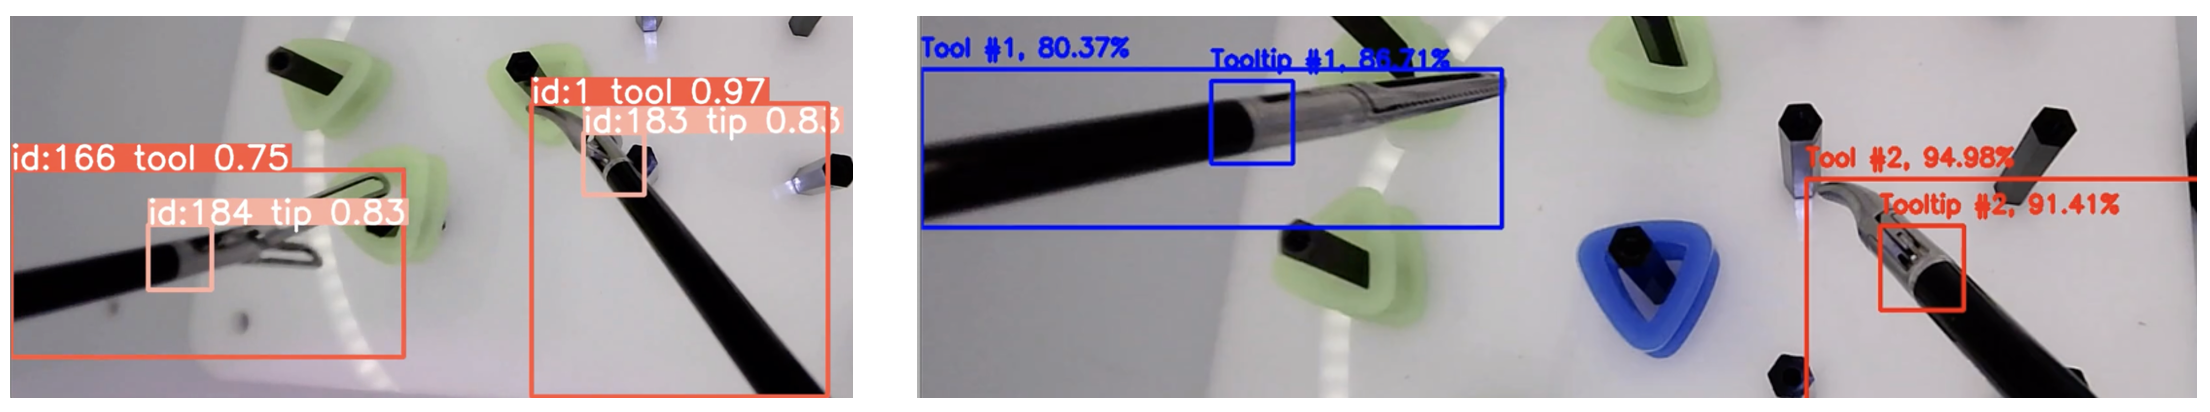
\includegraphics[width=1\linewidth]{test5_results.png}
    \vspace*{-7.5mm}
    \caption{Tool Detection and Tracking Results.}
    \vspace*{-6mm}
    \label{fig:test5_results}
    \Description{Tool Detection and Tracking Results using the YOLOv8-X model with YOLO tracking (left), in-house tracking (right) and original annotations (top).}
\end{figure}

\subsection{Model Usability}

The AI-ELT dataset differs significantly from in-vivo datasets, leading to better results due to more straightforward scenes and higher data quality. This is observed when comparing our investigation on the ART-Net dataset and against SOTA models on other datasets. However, the models' usability is focused on an in-vitro context, excluding the most well-known surgical and laparoscopic datasets. YOLO models showed rapid convergence to usable solutions and are lightweight (6.2MB weights for the smallest YOLOv8-N and 136.7MB for the largest YOLOv8-X) and run in real-time but may require testing on less capable hardware.

%Deploying a model on a server and using an Application Programming Interface (API) to interact by sending requests over the internet from even a mobile phone may be even more feasible in cases where establishing an internet connection would be cheaper than new hardware, especially if there are many surgical training bootcamp locations. In its current stage, the models' intended users would be researchers and developers. There would be no interaction with input data handling unless there is the intention to fine-tune a model for new datasets, such as with proprietary machines at a specific hospital.

\subsection{Limitations}

The models were trained using default configurations and not fine-tuned, implying that the results could have been better. Hyperparameter tuning and increased patience values could have improved results across all models. We tested a small number of models on only one other dataset. The AI-ELT dataset is extensive and of high quality, but it was collected from a single training event, and the tools are from a single manufacturer. This could introduce bias and not generalise well to other environments or tools. Human bias in labelling makes localisation results hard to evaluate quantitatively and fairly. Hardware used in this study may be more advanced than what will be available in LMICs.

\subsection{Comparison to Previous Work}

While there has been ample research on surgical tool detection and tracking, much less focus has been on using SOTA methods to explore new datasets for surgical training and skill assessment. This study evaluated some of the latest well-established models on a new, novel dataset and achieved exceptional detection and tracking results. However, our main aim was to focus on the AI-ELT dataset, so we did not endeavour to enhance existing scores or assess a wide range of datasets. Additionally, we have contributed valuable code to the limited existing resources and expect that the framework we have provided will facilitate future research. Our discussion comparing the results should also aid future work.

\subsection{Future Work}

With a new dataset, there is a plethora of potential for future work. By utilising the total degrees of freedom in the dataset, we could build a model to track the tools in three dimensions and estimate the tool poses, giving us a 3D spatial reconstruction of the tools and their movements. This would allow for a more accurate and robust tool tracking system, providing more accurate insights and increased reliability through minimised error in evaluating surgical skills. More standard and lightweight computer vision techniques can filter out parts of the scene and create better attention, reducing the model's inference time. Using the more precise tool detection results to crop search space for tooltip detection can improve precision and inference times. Models can be fine-tuned and tested on other datasets, especially with different tools, to compare the results with existing SOTA more quantitatively. The best model can weakly label all images with no bounding box annotations. Future data should be calibrated for exact sensor mapping within an image, as our localisation results were imperfect due to jittering. Annotations can be adapted so that the type of tool is labelled and can be classified, potentially helpful in predicting surgery workflow.

\subsection{Conclusion}
 
This study contributes to developing low-cost AI-driven intelligent systems that can easily be adapted to resource-constraint settings and set up in specialised surgical training programs to provide automated, personalised feedback to trainees. The AI-ELT dataset, particularly useful for applications in LMICs where access to advanced training facilities is limited, is comparable to what would be obtained in real-world training settings. Models were developed that can accurately and efficiently detect and track the position of surgical tools. The findings from the comparative analysis will inform the development of more generalisable models applicable to a wide range of laparoscopic procedures in in-vitro contexts.

% Surgical tool detection and tracking can be used to give live feedback to surgeons, in training contexts, by providing feedback to surgeons in past surgeries or for trainees on surgical training apparatus. 


\begin{acks}
O. Choudhry's Ph.D. studies is supported by the University of Leeds (UoL). The work was supported in full by UK Research and Innovation (UKRI) and UK Engineering and Physical Sciences Research Council (EPSRC) grant EP/S024336/1 for the UoL Centre for Doctoral Training in Artificial Intelligence for Medical Diagnosis and Care. Any opinions, findings, conclusions, or recommendations expressed in this article are those of the author and do not necessarily reflect the views of the UKRI, ESPRC or UoL.

We would like to thank the supervisors Dr Dominic Jones and Dr Sharib Ali for their guidance and support throughout the project.
\end{acks}

\section*{Reporting Statement}

In this paper we aim to follow the Transparent Reporting of a multivariable prediction model for Individual Prognosis Or Diagnosis (TRIPOD+AI) \cite{collins_tripodai_2024}, in order to assist in the reporting of this study. Even though we will not be looking specifically at prognosis or diagnosis, the TRIPOD+AI guidelines still provide a useful framework for the reporting of machine learning studies in healthcare.

\section*{Conflict of Interest Statement}

The authors declare no conflicts of interest.

\section*{Ethical Approval Statement}

This study was approved by the University of Leeds School of Computing Ethics Committee. \textcolor{red}{(Approval number: \textit{[insert number here]})}.

\section*{Data Availability Statement}

The in-house dataset is publically available at the repository: \url{https://github.com/omariosc/msc-surgical-tool-tracking/}. The ART-Net dataset can be requested from the authors of the original paper in the following repository: \url{https://github.com/kamruleee51/ART-Net}. \cite{hasan_detection_2021}.

\section*{Code Sharing Statement}

The code, including all helper files, scripts, notebooks, models and checkpoints used in this study are all freely available at the repository: \url{https://github.com/omariosc/msc-surgical-tool-tracking/}.

%%
%% The next two lines define the bibliography style to be used, and
%% the bibliography file.
\bibliographystyle{ACM-Reference-Format}
\bibliography{sample-base}


%%
%% If your work has an appendix, this is the place to put it.
\appendix

\section{Research Methods}

\subsection{Part One}



\subsection{Part Two}



\section{Online Resources}



\end{document}
\endinput
%%
%% End of file `sample-sigconf-authordraft.tex'.

% %%
% %% This is file `sample-sigconf-authordraft.tex',
% %% generated with the docstrip utility.
% %%
% %% The original source files were:
% %%
% %% samples.dtx  (with options: `all,proceedings,bibtex,authordraft')
% %% 
% %% IMPORTANT NOTICE:
% %% 
% %% For the copyright see the source file.
% %% 
% %% Any modified versions of this file must be renamed
% %% with new filenames distinct from sample-sigconf-authordraft.tex.
% %% 
% %% For distribution of the original source see the terms
% %% for copying and modification in the file samples.dtx.
% %% 
% %% This generated file may be distributed as long as the
% %% original source files, as listed above, are part of the
% %% same distribution. (The sources need not necessarily be
% %% in the same archive or directory.)
% %%
% %%
% %% Commands for TeXCount
% %TC:macro \cite [option:text,text]
% %TC:macro \citep [option:text,text]
% %TC:macro \citet [option:text,text]
% %TC:envir table 0 1
% %TC:envir table* 0 1
% %TC:envir tabular [ignore] word
% %TC:envir displaymath 0 word
% %TC:envir math 0 word
% %TC:envir comment 0 0
% %%
% %%
% %% The first command in your LaTeX source must be the \documentclass
% %% command.
% %%
% %% For submission and review of your manuscript please change the
% %% command to \documentclass[manuscript, screen, review]{acmart}.
% %%
% %% When submitting camera ready or to TAPS, please change the command
% %% to \documentclass[sigconf]{acmart} or whichever template is required
% %% for your publication.
% %%
% %%
% \documentclass[sigconf,authordraft]{acmart}

% %%
% %% \BibTeX command to typeset BibTeX logo in the docs
% \AtBeginDocument{%
%   \providecommand\BibTeX{{%
%     Bib\TeX}}}

% %% Rights management information.  This information is sent to you
% %% when you complete the rights form.  These commands have SAMPLE
% %% values in them; it is your responsibility as an author to replace
% %% the commands and values with those provided to you when you
% %% complete the rights form.
% \setcopyright{acmlicensed}
% \copyrightyear{2018}
% \acmYear{2018}
% \acmDOI{XXXXXXX.XXXXXXX}

% %% These commands are for a PROCEEDINGS abstract or paper.
% \acmConference[Conference acronym 'XX]{Make sure to enter the correct
%   conference title from your rights confirmation emai}{June 03--05,
%   2018}{Woodstock, NY}
% %%
% %%  Uncomment \acmBooktitle if the title of the proceedings is different
% %%  from ``Proceedings of ...''!
% %%
% %%\acmBooktitle{Woodstock '18: ACM Symposium on Neural Gaze Detection,
% %%  June 03--05, 2018, Woodstock, NY}
% \acmISBN{978-1-4503-XXXX-X/18/06}


% %%
% %% Submission ID.
% %% Use this when submitting an article to a sponsored event. You'll
% %% receive a unique submission ID from the organizers
% %% of the event, and this ID should be used as the parameter to this command.
% %%\acmSubmissionID{123-A56-BU3}

% %%
% %% For managing citations, it is recommended to use bibliography
% %% files in BibTeX format.
% %%
% %% You can then either use BibTeX with the ACM-Reference-Format style,
% %% or BibLaTeX with the acmnumeric or acmauthoryear sytles, that include
% %% support for advanced citation of software artefact from the
% %% biblatex-software package, also separately available on CTAN.
% %%
% %% Look at the sample-*-biblatex.tex files for templates showcasing
% %% the biblatex styles.
% %%

% %%
% %% The majority of ACM publications use numbered citations and
% %% references.  The command \citestyle{authoryear} switches to the
% %% "author year" style.
% %%
% %% If you are preparing content for an event
% %% sponsored by ACM SIGGRAPH, you must use the "author year" style of
% %% citations and references.
% %% Uncommenting
% %% the next command will enable that style.
% %%\citestyle{acmauthoryear}


% %%
% %% end of the preamble, start of the body of the document source.
% \begin{document}

% %%
% %% The "title" command has an optional parameter,
% %% allowing the author to define a "short title" to be used in page headers.
% \title{The Name of the Title Is Hope}

% %%
% %% The "author" command and its associated commands are used to define
% %% the authors and their affiliations.
% %% Of note is the shared affiliation of the first two authors, and the
% %% "authornote" and "authornotemark" commands
% %% used to denote shared contribution to the research.
% \author{Ben Trovato}
% \authornote{Both authors contributed equally to this research.}
% \email{trovato@corporation.com}
% \orcid{1234-5678-9012}
% \author{G.K.M. Tobin}
% \authornotemark[1]
% \email{webmaster@marysville-ohio.com}
% \affiliation{%
%   \institution{Institute for Clarity in Documentation}
%   \city{Dublin}
%   \state{Ohio}
%   \country{USA}
% }

% \author{Lars Th{\o}rv{\"a}ld}
% \affiliation{%
%   \institution{The Th{\o}rv{\"a}ld Group}
%   \city{Hekla}
%   \country{Iceland}}
% \email{larst@affiliation.org}

% \author{Valerie B\'eranger}
% \affiliation{%
%   \institution{Inria Paris-Rocquencourt}
%   \city{Rocquencourt}
%   \country{France}
% }

% \author{Aparna Patel}
% \affiliation{%
%  \institution{Rajiv Gandhi University}
%  \city{Doimukh}
%  \state{Arunachal Pradesh}
%  \country{India}}

% \author{Huifen Chan}
% \affiliation{%
%   \institution{Tsinghua University}
%   \city{Haidian Qu}
%   \state{Beijing Shi}
%   \country{China}}

% \author{Charles Palmer}
% \affiliation{%
%   \institution{Palmer Research Laboratories}
%   \city{San Antonio}
%   \state{Texas}
%   \country{USA}}
% \email{cpalmer@prl.com}

% \author{John Smith}
% \affiliation{%
%   \institution{The Th{\o}rv{\"a}ld Group}
%   \city{Hekla}
%   \country{Iceland}}
% \email{jsmith@affiliation.org}

% \author{Julius P. Kumquat}
% \affiliation{%
%   \institution{The Kumquat Consortium}
%   \city{New York}
%   \country{USA}}
% \email{jpkumquat@consortium.net}

% %%
% %% By default, the full list of authors will be used in the page
% %% headers. Often, this list is too long, and will overlap
% %% other information printed in the page headers. This command allows
% %% the author to define a more concise list
% %% of authors' names for this purpose.
% \renewcommand{\shortauthors}{Trovato et al.}

% %%
% %% The abstract is a short summary of the work to be presented in the
% %% article.
% \begin{abstract}
%   A clear and well-documented \LaTeX\ document is presented as an
%   article formatted for publication by ACM in a conference proceedings
%   or journal publication. Based on the ``acmart'' document class, this
%   article presents and explains many of the common variations, as well
%   as many of the formatting elements an author may use in the
%   preparation of the documentation of their work.
% \end{abstract}

% %%
% %% The code below is generated by the tool at http://dl.acm.org/ccs.cfm.
% %% Please copy and paste the code instead of the example below.
% %%
% \begin{CCSXML}
% <ccs2012>
%  <concept>
%   <concept_id>00000000.0000000.0000000</concept_id>
%   <concept_desc>Do Not Use This Code, Generate the Correct Terms for Your Paper</concept_desc>
%   <concept_significance>500</concept_significance>
%  </concept>
%  <concept>
%   <concept_id>00000000.00000000.00000000</concept_id>
%   <concept_desc>Do Not Use This Code, Generate the Correct Terms for Your Paper</concept_desc>
%   <concept_significance>300</concept_significance>
%  </concept>
%  <concept>
%   <concept_id>00000000.00000000.00000000</concept_id>
%   <concept_desc>Do Not Use This Code, Generate the Correct Terms for Your Paper</concept_desc>
%   <concept_significance>100</concept_significance>
%  </concept>
%  <concept>
%   <concept_id>00000000.00000000.00000000</concept_id>
%   <concept_desc>Do Not Use This Code, Generate the Correct Terms for Your Paper</concept_desc>
%   <concept_significance>100</concept_significance>
%  </concept>
% </ccs2012>
% \end{CCSXML}

% \ccsdesc[500]{Do Not Use This Code~Generate the Correct Terms for Your Paper}
% \ccsdesc[300]{Do Not Use This Code~Generate the Correct Terms for Your Paper}
% \ccsdesc{Do Not Use This Code~Generate the Correct Terms for Your Paper}
% \ccsdesc[100]{Do Not Use This Code~Generate the Correct Terms for Your Paper}

% %%
% %% Keywords. The author(s) should pick words that accurately describe
% %% the work being presented. Separate the keywords with commas.
% \keywords{Do, Not, Us, This, Code, Put, the, Correct, Terms, for,
%   Your, Paper}
% %% A "teaser" image appears between the author and affiliation
% %% information and the body of the document, and typically spans the
% %% page.
% \begin{teaserfigure}
%   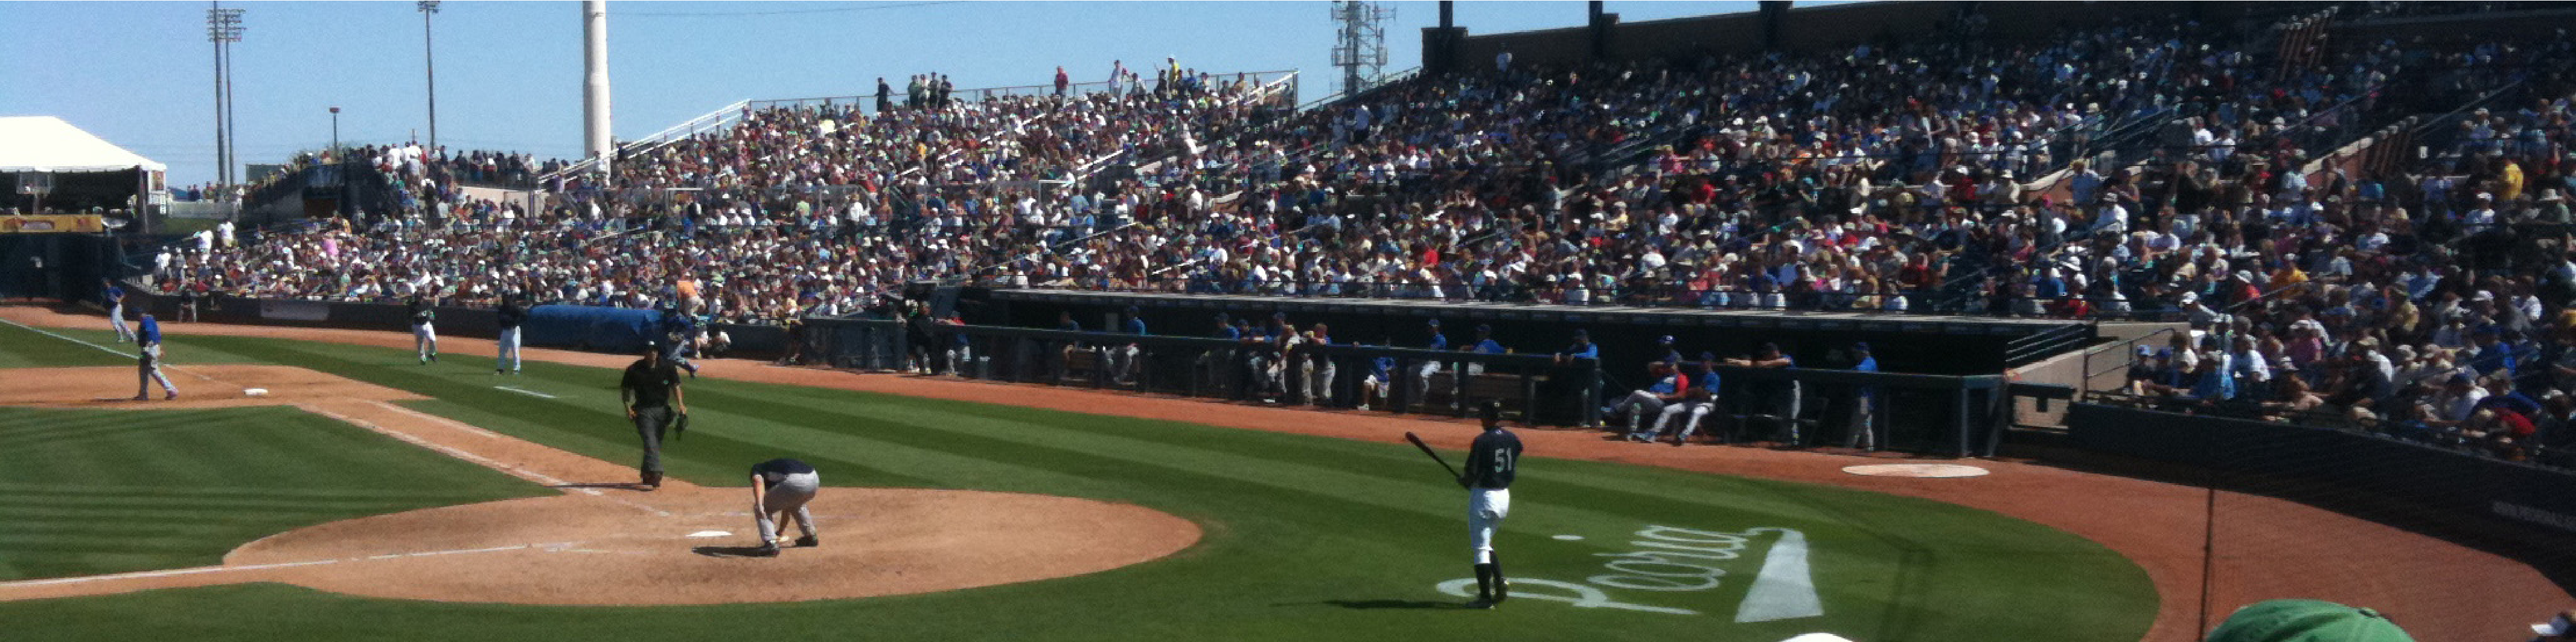
\includegraphics[width=\textwidth]{sampleteaser}
%   \caption{Seattle Mariners at Spring Training, 2010.}
%   \Description{Enjoying the baseball game from the third-base
%   seats. Ichiro Suzuki preparing to bat.}
%   \label{fig:teaser}
% \end{teaserfigure}

% \received{20 February 2007}
% \received[revised]{12 March 2009}
% \received[accepted]{5 June 2009}

% %%
% %% This command processes the author and affiliation and title
% %% information and builds the first part of the formatted document.
% \maketitle

% \section{Introduction}
% ACM's consolidated article template, introduced in 2017, provides a
% consistent \LaTeX\ style for use across ACM publications, and
% incorporates accessibility and metadata-extraction functionality
% necessary for future Digital Library endeavors. Numerous ACM and
% SIG-specific \LaTeX\ templates have been examined, and their unique
% features incorporated into this single new template.

% If you are new to publishing with ACM, this document is a valuable
% guide to the process of preparing your work for publication. If you
% have published with ACM before, this document provides insight and
% instruction into more recent changes to the article template.

% The ``\verb|acmart|'' document class can be used to prepare articles
% for any ACM publication --- conference or journal, and for any stage
% of publication, from review to final ``camera-ready'' copy, to the
% author's own version, with {\itshape very} few changes to the source.

% \section{Template Overview}
% As noted in the introduction, the ``\verb|acmart|'' document class can
% be used to prepare many different kinds of documentation --- a
% double-anonymous initial submission of a full-length technical paper, a
% two-page SIGGRAPH Emerging Technologies abstract, a ``camera-ready''
% journal article, a SIGCHI Extended Abstract, and more --- all by
% selecting the appropriate {\itshape template style} and {\itshape
%   template parameters}.

% This document will explain the major features of the document
% class. For further information, the {\itshape \LaTeX\ User's Guide} is
% available from
% \url{https://www.acm.org/publications/proceedings-template}.

% \subsection{Template Styles}

% The primary parameter given to the ``\verb|acmart|'' document class is
% the {\itshape template style} which corresponds to the kind of publication
% or SIG publishing the work. This parameter is enclosed in square
% brackets and is a part of the {\verb|documentclass|} command:
% \begin{verbatim}
%   \documentclass[STYLE]{acmart}
% \end{verbatim}

% Journals use one of three template styles. All but three ACM journals
% use the {\verb|acmsmall|} template style:
% \begin{itemize}
% \item {\texttt{acmsmall}}: The default journal template style.
% \item {\texttt{acmlarge}}: Used by JOCCH and TAP.
% \item {\texttt{acmtog}}: Used by TOG.
% \end{itemize}

% The majority of conference proceedings documentation will use the {\verb|acmconf|} template style.
% \begin{itemize}
% \item {\texttt{sigconf}}: The default proceedings template style.
% \item{\texttt{sigchi}}: Used for SIGCHI conference articles.
% \item{\texttt{sigplan}}: Used for SIGPLAN conference articles.
% \end{itemize}

% \subsection{Template Parameters}

% In addition to specifying the {\itshape template style} to be used in
% formatting your work, there are a number of {\itshape template parameters}
% which modify some part of the applied template style. A complete list
% of these parameters can be found in the {\itshape \LaTeX\ User's Guide.}

% Frequently-used parameters, or combinations of parameters, include:
% \begin{itemize}
% \item {\texttt{anonymous,review}}: Suitable for a ``double-anonymous''
%   conference submission. Anonymizes the work and includes line
%   numbers. Use with the \texttt{\acmSubmissionID} command to print the
%   submission's unique ID on each page of the work.
% \item{\texttt{authorversion}}: Produces a version of the work suitable
%   for posting by the author.
% \item{\texttt{screen}}: Produces colored hyperlinks.
% \end{itemize}

% This document uses the following string as the first command in the
% source file:
% \begin{verbatim}
% \documentclass[sigconf,authordraft]{acmart}
% \end{verbatim}

% \section{Modifications}

% Modifying the template --- including but not limited to: adjusting
% margins, typeface sizes, line spacing, paragraph and list definitions,
% and the use of the \verb|\vspace| command to manually adjust the
% vertical spacing between elements of your work --- is not allowed.

% {\bfseries Your document will be returned to you for revision if
%   modifications are discovered.}

% \section{Typefaces}

% The ``\verb|acmart|'' document class requires the use of the
% ``Libertine'' typeface family. Your \TeX\ installation should include
% this set of packages. Please do not substitute other typefaces. The
% ``\verb|lmodern|'' and ``\verb|ltimes|'' packages should not be used,
% as they will override the built-in typeface families.

% \section{Title Information}

% The title of your work should use capital letters appropriately -
% \url{https://capitalizemytitle.com/} has useful rules for
% capitalization. Use the {\verb|title|} command to define the title of
% your work. If your work has a subtitle, define it with the
% {\verb|subtitle|} command.  Do not insert line breaks in your title.

% If your title is lengthy, you must define a short version to be used
% in the page headers, to prevent overlapping text. The \verb|title|
% command has a ``short title'' parameter:
% \begin{verbatim}
%   \title[short title]{full title}
% \end{verbatim}

% \section{Authors and Affiliations}

% Each author must be defined separately for accurate metadata
% identification.  As an exception, multiple authors may share one
% affiliation. Authors' names should not be abbreviated; use full first
% names wherever possible. Include authors' e-mail addresses whenever
% possible.

% Grouping authors' names or e-mail addresses, or providing an ``e-mail
% alias,'' as shown below, is not acceptable:
% \begin{verbatim}
%   \author{Brooke Aster, David Mehldau}
%   \email{dave,judy,steve@university.edu}
%   \email{firstname.lastname@phillips.org}
% \end{verbatim}

% The \verb|authornote| and \verb|authornotemark| commands allow a note
% to apply to multiple authors --- for example, if the first two authors
% of an article contributed equally to the work.

% If your author list is lengthy, you must define a shortened version of
% the list of authors to be used in the page headers, to prevent
% overlapping text. The following command should be placed just after
% the last \verb|\author{}| definition:
% \begin{verbatim}
%   \renewcommand{\shortauthors}{McCartney, et al.}
% \end{verbatim}
% Omitting this command will force the use of a concatenated list of all
% of the authors' names, which may result in overlapping text in the
% page headers.

% The article template's documentation, available at
% \url{https://www.acm.org/publications/proceedings-template}, has a
% complete explanation of these commands and tips for their effective
% use.

% Note that authors' addresses are mandatory for journal articles.

% \section{Rights Information}

% Authors of any work published by ACM will need to complete a rights
% form. Depending on the kind of work, and the rights management choice
% made by the author, this may be copyright transfer, permission,
% license, or an OA (open access) agreement.

% Regardless of the rights management choice, the author will receive a
% copy of the completed rights form once it has been submitted. This
% form contains \LaTeX\ commands that must be copied into the source
% document. When the document source is compiled, these commands and
% their parameters add formatted text to several areas of the final
% document:
% \begin{itemize}
% \item the ``ACM Reference Format'' text on the first page.
% \item the ``rights management'' text on the first page.
% \item the conference information in the page header(s).
% \end{itemize}

% Rights information is unique to the work; if you are preparing several
% works for an event, make sure to use the correct set of commands with
% each of the works.

% The ACM Reference Format text is required for all articles over one
% page in length, and is optional for one-page articles (abstracts).

% \section{CCS Concepts and User-Defined Keywords}

% Two elements of the ``acmart'' document class provide powerful
% taxonomic tools for you to help readers find your work in an online
% search.

% The ACM Computing Classification System ---
% \url{https://www.acm.org/publications/class-2012} --- is a set of
% classifiers and concepts that describe the computing
% discipline. Authors can select entries from this classification
% system, via \url{https://dl.acm.org/ccs/ccs.cfm}, and generate the
% commands to be included in the \LaTeX\ source.

% User-defined keywords are a comma-separated list of words and phrases
% of the authors' choosing, providing a more flexible way of describing
% the research being presented.

% CCS concepts and user-defined keywords are required for for all
% articles over two pages in length, and are optional for one- and
% two-page articles (or abstracts).

% \section{Sectioning Commands}

% Your work should use standard \LaTeX\ sectioning commands:
% \verb|section|, \verb|subsection|, \verb|subsubsection|, and
% \verb|paragraph|. They should be numbered; do not remove the numbering
% from the commands.

% Simulating a sectioning command by setting the first word or words of
% a paragraph in boldface or italicized text is {\bfseries not allowed.}

% \section{Tables}

% The ``\verb|acmart|'' document class includes the ``\verb|booktabs|''
% package --- \url{https://ctan.org/pkg/booktabs} --- for preparing
% high-quality tables.

% Table captions are placed {\itshape above} the table.

% Because tables cannot be split across pages, the best placement for
% them is typically the top of the page nearest their initial cite.  To
% ensure this proper ``floating'' placement of tables, use the
% environment \textbf{table} to enclose the table's contents and the
% table caption.  The contents of the table itself must go in the
% \textbf{tabular} environment, to be aligned properly in rows and
% columns, with the desired horizontal and vertical rules.  Again,
% detailed instructions on \textbf{tabular} material are found in the
% \textit{\LaTeX\ User's Guide}.

% Immediately following this sentence is the point at which
% Table~\ref{tab:freq} is included in the input file; compare the
% placement of the table here with the table in the printed output of
% this document.

% \begin{table}
%   \caption{Frequency of Special Characters}
%   \label{tab:freq}
%   \begin{tabular}{ccl}
%     \toprule
%     Non-English or Math&Frequency&Comments\\
%     \midrule
%     \O & 1 in 1,000& For Swedish names\\
%     $\pi$ & 1 in 5& Common in math\\
%     \$ & 4 in 5 & Used in business\\
%     $\Psi^2_1$ & 1 in 40,000& Unexplained usage\\
%   \bottomrule
% \end{tabular}
% \end{table}

% To set a wider table, which takes up the whole width of the page's
% live area, use the environment \textbf{table*} to enclose the table's
% contents and the table caption.  As with a single-column table, this
% wide table will ``float'' to a location deemed more
% desirable. Immediately following this sentence is the point at which
% Table~\ref{tab:commands} is included in the input file; again, it is
% instructive to compare the placement of the table here with the table
% in the printed output of this document.

% \begin{table*}
%   \caption{Some Typical Commands}
%   \label{tab:commands}
%   \begin{tabular}{ccl}
%     \toprule
%     Command &A Number & Comments\\
%     \midrule
%     \texttt{{\char'134}author} & 100& Author \\
%     \texttt{{\char'134}table}& 300 & For tables\\
%     \texttt{{\char'134}table*}& 400& For wider tables\\
%     \bottomrule
%   \end{tabular}
% \end{table*}

% Always use midrule to separate table header rows from data rows, and
% use it only for this purpose. This enables assistive technologies to
% recognise table headers and support their users in navigating tables
% more easily.

% \section{Math Equations}
% You may want to display math equations in three distinct styles:
% inline, numbered or non-numbered display.  Each of the three are
% discussed in the next sections.

% \subsection{Inline (In-text) Equations}
% A formula that appears in the running text is called an inline or
% in-text formula.  It is produced by the \textbf{math} environment,
% which can be invoked with the usual
% \texttt{{\char'134}begin\,\ldots{\char'134}end} construction or with
% the short form \texttt{\$\,\ldots\$}. You can use any of the symbols
% and structures, from $\alpha$ to $\omega$, available in
% \LaTeX~\cite{Lamport:LaTeX}; this section will simply show a few
% examples of in-text equations in context. Notice how this equation:
% \begin{math}
%   \lim_{n\rightarrow \infty}x=0
% \end{math},
% set here in in-line math style, looks slightly different when
% set in display style.  (See next section).

% \subsection{Display Equations}
% A numbered display equation---one set off by vertical space from the
% text and centered horizontally---is produced by the \textbf{equation}
% environment. An unnumbered display equation is produced by the
% \textbf{displaymath} environment.

% Again, in either environment, you can use any of the symbols and
% structures available in \LaTeX\@; this section will just give a couple
% of examples of display equations in context.  First, consider the
% equation, shown as an inline equation above:
% \begin{equation}
%   \lim_{n\rightarrow \infty}x=0
% \end{equation}
% Notice how it is formatted somewhat differently in
% the \textbf{displaymath}
% environment.  Now, we'll enter an unnumbered equation:
% \begin{displaymath}
%   \sum_{i=0}^{\infty} x + 1
% \end{displaymath}
% and follow it with another numbered equation:
% \begin{equation}
%   \sum_{i=0}^{\infty}x_i=\int_{0}^{\pi+2} f
% \end{equation}
% just to demonstrate \LaTeX's able handling of numbering.

% \section{Figures}

% The ``\verb|figure|'' environment should be used for figures. One or
% more images can be placed within a figure. If your figure contains
% third-party material, you must clearly identify it as such, as shown
% in the example below.
% \begin{figure}[h]
%   \centering
%   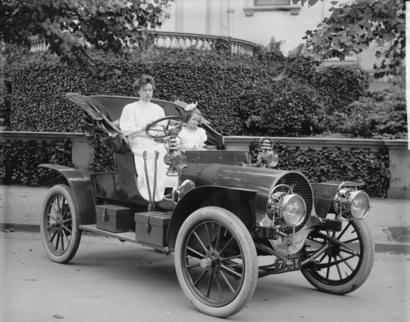
\includegraphics[width=\linewidth]{sample-franklin}
%   \caption{1907 Franklin Model D roadster. Photograph by Harris \&
%     Ewing, Inc. [Public domain], via Wikimedia
%     Commons. (\url{https://goo.gl/VLCRBB}).}
%   \Description{A woman and a girl in white dresses sit in an open car.}
% \end{figure}

% Your figures should contain a caption which describes the figure to
% the reader.

% Figure captions are placed {\itshape below} the figure.

% Every figure should also have a figure description unless it is purely
% decorative. These descriptions convey what’s in the image to someone
% who cannot see it. They are also used by search engine crawlers for
% indexing images, and when images cannot be loaded.

% A figure description must be unformatted plain text less than 2000
% characters long (including spaces).  {\bfseries Figure descriptions
%   should not repeat the figure caption – their purpose is to capture
%   important information that is not already provided in the caption or
%   the main text of the paper.} For figures that convey important and
% complex new information, a short text description may not be
% adequate. More complex alternative descriptions can be placed in an
% appendix and referenced in a short figure description. For example,
% provide a data table capturing the information in a bar chart, or a
% structured list representing a graph.  For additional information
% regarding how best to write figure descriptions and why doing this is
% so important, please see
% \url{https://www.acm.org/publications/taps/describing-figures/}.

% \subsection{The ``Teaser Figure''}

% A ``teaser figure'' is an image, or set of images in one figure, that
% are placed after all author and affiliation information, and before
% the body of the article, spanning the page. If you wish to have such a
% figure in your article, place the command immediately before the
% \verb|\maketitle| command:
% \begin{verbatim}
%   \begin{teaserfigure}
%     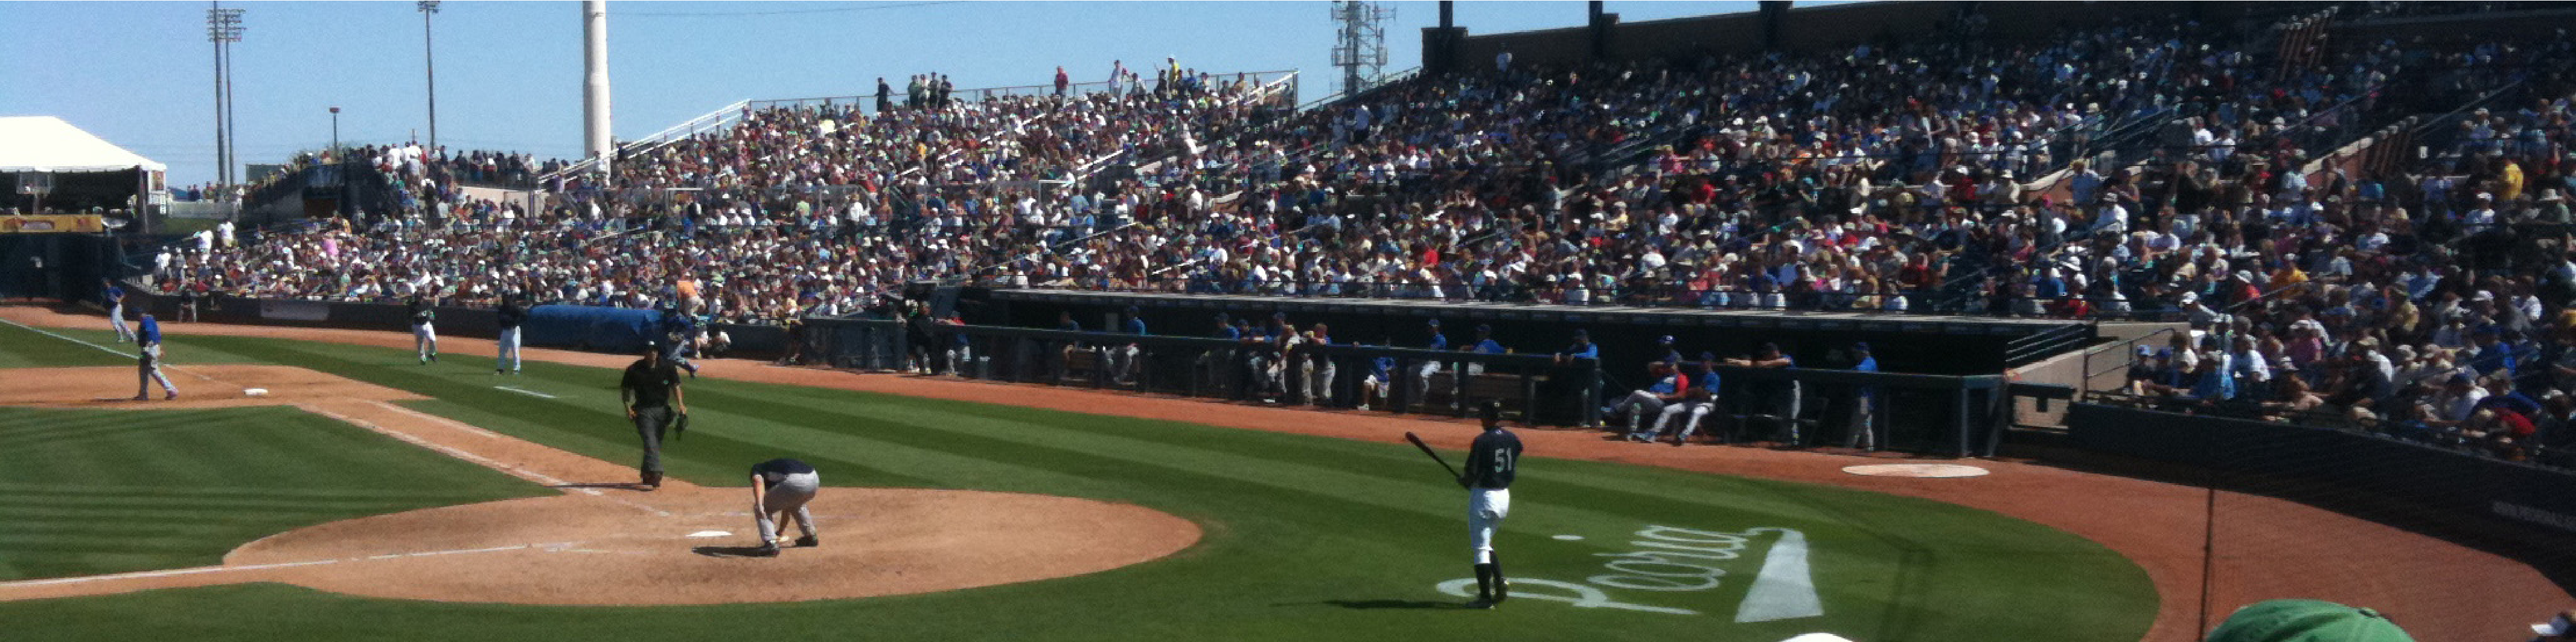
\includegraphics[width=\textwidth]{sampleteaser}
%     \caption{figure caption}
%     \Description{figure description}
%   \end{teaserfigure}
% \end{verbatim}

% \section{Citations and Bibliographies}

% The use of \BibTeX\ for the preparation and formatting of one's
% references is strongly recommended. Authors' names should be complete
% --- use full first names (``Donald E. Knuth'') not initials
% (``D. E. Knuth'') --- and the salient identifying features of a
% reference should be included: title, year, volume, number, pages,
% article DOI, etc.

% The bibliography is included in your source document with these two
% commands, placed just before the \verb|\end{document}| command:
% \begin{verbatim}
%   \bibliographystyle{ACM-Reference-Format}
%   \bibliography{bibfile}
% \end{verbatim}
% where ``\verb|bibfile|'' is the name, without the ``\verb|.bib|''
% suffix, of the \BibTeX\ file.

% Citations and references are numbered by default. A small number of
% ACM publications have citations and references formatted in the
% ``author year'' style; for these exceptions, please include this
% command in the {\bfseries preamble} (before the command
% ``\verb|\begin{document}|'') of your \LaTeX\ source:
% \begin{verbatim}
%   \citestyle{acmauthoryear}
% \end{verbatim}


%   Some examples.  A paginated journal article \cite{Abril07}, an
%   enumerated journal article \cite{Cohen07}, a reference to an entire
%   issue \cite{JCohen96}, a monograph (whole book) \cite{Kosiur01}, a
%   monograph/whole book in a series (see 2a in spec. document)
%   \cite{Harel79}, a divisible-book such as an anthology or compilation
%   \cite{Editor00} followed by the same example, however we only output
%   the series if the volume number is given \cite{Editor00a} (so
%   Editor00a's series should NOT be present since it has no vol. no.),
%   a chapter in a divisible book \cite{Spector90}, a chapter in a
%   divisible book in a series \cite{Douglass98}, a multi-volume work as
%   book \cite{Knuth97}, a couple of articles in a proceedings (of a
%   conference, symposium, workshop for example) (paginated proceedings
%   article) \cite{Andler79, Hagerup1993}, a proceedings article with
%   all possible elements \cite{Smith10}, an example of an enumerated
%   proceedings article \cite{VanGundy07}, an informally published work
%   \cite{Harel78}, a couple of preprints \cite{Bornmann2019,
%     AnzarootPBM14}, a doctoral dissertation \cite{Clarkson85}, a
%   master's thesis: \cite{anisi03}, an online document / world wide web
%   resource \cite{Thornburg01, Ablamowicz07, Poker06}, a video game
%   (Case 1) \cite{Obama08} and (Case 2) \cite{Novak03} and \cite{Lee05}
%   and (Case 3) a patent \cite{JoeScientist001}, work accepted for
%   publication \cite{rous08}, 'YYYYb'-test for prolific author
%   \cite{SaeediMEJ10} and \cite{SaeediJETC10}. Other cites might
%   contain 'duplicate' DOI and URLs (some SIAM articles)
%   \cite{Kirschmer:2010:AEI:1958016.1958018}. Boris / Barbara Beeton:
%   multi-volume works as books \cite{MR781536} and \cite{MR781537}. A
%   couple of citations with DOIs:
%   \cite{2004:ITE:1009386.1010128,Kirschmer:2010:AEI:1958016.1958018}. Online
%   citations: \cite{TUGInstmem, Thornburg01, CTANacmart}.
%   Artifacts: \cite{R} and \cite{UMassCitations}.

% \section{Acknowledgments}

% Identification of funding sources and other support, and thanks to
% individuals and groups that assisted in the research and the
% preparation of the work should be included in an acknowledgment
% section, which is placed just before the reference section in your
% document.

% This section has a special environment:
% \begin{verbatim}
%   \begin{acks}
%   ...
%   \end{acks}
% \end{verbatim}
% so that the information contained therein can be more easily collected
% during the article metadata extraction phase, and to ensure
% consistency in the spelling of the section heading.

% Authors should not prepare this section as a numbered or unnumbered {\verb|\section|}; please use the ``{\verb|acks|}'' environment.

% \section{Appendices}

% If your work needs an appendix, add it before the
% ``\verb|\end{document}|'' command at the conclusion of your source
% document.

% Start the appendix with the ``\verb|appendix|'' command:
% \begin{verbatim}
%   \appendix
% \end{verbatim}
% and note that in the appendix, sections are lettered, not
% numbered. This document has two appendices, demonstrating the section
% and subsection identification method.

% \section{Multi-language papers}

% Papers may be written in languages other than English or include
% titles, subtitles, keywords and abstracts in different languages (as a
% rule, a paper in a language other than English should include an
% English title and an English abstract).  Use \verb|language=...| for
% every language used in the paper.  The last language indicated is the
% main language of the paper.  For example, a French paper with
% additional titles and abstracts in English and German may start with
% the following command
% \begin{verbatim}
% \documentclass[sigconf, language=english, language=german,
%                language=french]{acmart}
% \end{verbatim}

% The title, subtitle, keywords and abstract will be typeset in the main
% language of the paper.  The commands \verb|\translatedXXX|, \verb|XXX|
% begin title, subtitle and keywords, can be used to set these elements
% in the other languages.  The environment \verb|translatedabstract| is
% used to set the translation of the abstract.  These commands and
% environment have a mandatory first argument: the language of the
% second argument.  See \verb|sample-sigconf-i13n.tex| file for examples
% of their usage.

% \section{SIGCHI Extended Abstracts}

% The ``\verb|sigchi-a|'' template style (available only in \LaTeX\ and
% not in Word) produces a landscape-orientation formatted article, with
% a wide left margin. Three environments are available for use with the
% ``\verb|sigchi-a|'' template style, and produce formatted output in
% the margin:
% \begin{description}
% \item[\texttt{sidebar}:]  Place formatted text in the margin.
% \item[\texttt{marginfigure}:] Place a figure in the margin.
% \item[\texttt{margintable}:] Place a table in the margin.
% \end{description}

% %%
% %% The acknowledgments section is defined using the "acks" environment
% %% (and NOT an unnumbered section). This ensures the proper
% %% identification of the section in the article metadata, and the
% %% consistent spelling of the heading.
% \begin{acks}
% To Robert, for the bagels and explaining CMYK and color spaces.
% \end{acks}

% %%
% %% The next two lines define the bibliography style to be used, and
% %% the bibliography file.
% \bibliographystyle{ACM-Reference-Format}
% \bibliography{sample-base}


% %%
% %% If your work has an appendix, this is the place to put it.
% \appendix

% \section{Research Methods}

% \subsection{Part One}

% Lorem ipsum dolor sit amet, consectetur adipiscing elit. Morbi
% malesuada, quam in pulvinar varius, metus nunc fermentum urna, id
% sollicitudin purus odio sit amet enim. Aliquam ullamcorper eu ipsum
% vel mollis. Curabitur quis dictum nisl. Phasellus vel semper risus, et
% lacinia dolor. Integer ultricies commodo sem nec semper.

% \subsection{Part Two}

% Etiam commodo feugiat nisl pulvinar pellentesque. Etiam auctor sodales
% ligula, non varius nibh pulvinar semper. Suspendisse nec lectus non
% ipsum convallis congue hendrerit vitae sapien. Donec at laoreet
% eros. Vivamus non purus placerat, scelerisque diam eu, cursus
% ante. Etiam aliquam tortor auctor efficitur mattis.

% \section{Online Resources}

% Nam id fermentum dui. Suspendisse sagittis tortor a nulla mollis, in
% pulvinar ex pretium. Sed interdum orci quis metus euismod, et sagittis
% enim maximus. Vestibulum gravida massa ut felis suscipit
% congue. Quisque mattis elit a risus ultrices commodo venenatis eget
% dui. Etiam sagittis eleifend elementum.

% Nam interdum magna at lectus dignissim, ac dignissim lorem
% rhoncus. Maecenas eu arcu ac neque placerat aliquam. Nunc pulvinar
% massa et mattis lacinia.

% \end{document}
% \endinput
% %%
% %% End of file `sample-sigconf-authordraft.tex'.
